% --------------------------------------------------------------------------- %
% --------------------------------------------------------------------------- %
\chapter{Missing Transverse Momentum}
\label{ch:MET}
% --------------------------------------------------------------------------- %
% --------------------------------------------------------------------------- %
In the final state targeted by this analysis, large values of \MET\ can arise from the LSP escaping detection.
It is important that \MET\ from standard model processes is predicted accurately.
\MET\ can be calculated using the full collection of PF candidates described in section~\ref{subs:particleflow}.
In the following sections, \MET\ calculations and corrections are described in detail.

\section{raw MET}

Calculating \MET\ using PF candidates is done by summing the transverse momentum vectors of all the PF candidates, described in equation~\ref{eqn:rawmet}.

\begin{equation}
  \label{eqn:rawmet}
\mathrm{E_{T}^{miss} = -|\sum_{i}\overrightarrow{p}_{T}^{i}|}
\end{equation}

When \MET\ is calculated without any calibration applied to the pf candidates, it is known as raw MET.

\section{Corrections to MET}
\MET\ comes from three main sources, resolution effects due to mismeasurement of physics objects (referred to as fake \MET),
particles escaping detection in the detector (for example by being too far forward in $\eta$ to be within the detector geometry),
and real physics process where particles do not interact with the detector, thereby escaping detection.
In the third case, the particles that are not detected can be standard model neutrinos, or particles from BSM theories such as the $\mathrm{\tilde{G}}$.
Since this analysis is searching in regions with large \MET, it is very important to be able to identify and measure backgrounds with fake \MET and real \MET.

When calculating \MET, the total contribution from pileup should be balanced since it is essentially random noise.
Pileup energy is removed from each jet's cone when the L1 correction is applied to the jet which creates an imbalance of \MET.
The imbalance is corrected by adding this energy back in, and this is called the Type 1 correction.

{\bf add plot with metx mety etc}

\section{Type 1 MET}
\label{sec:t1met}
Type 1 \MET\ refers to a version of \MET\ where the corrections that are applied to jets are propagated to the \MET\ calculation as described in section~\ref{ssec:jets}.
The correction factors applied to the jets are derived for jets down to 10 \gev.
The way these corrections are propagated to the \MET\ is not as straightforward as just adding the corrections vectorially with the \MET.

The jets we use in this analysis are made using all the pf candidates, except the charged pf candidates that are not associated with the primary vertex.
Leptons and photons are included in the collection of pf candidates used when clustering jets.
The jet corrections are meant to correct jets that come from hadronic objects, such as quarks and gluons.
If the jet corrections are applied to lepton and photon objects, the
The jet corrections are not meant to be applied to lepton and photon objects.
When propagating the jet corrections to the \MET, we exclude corrections on jets with an electromagnetic fraction larger than 90\%,
and remove the pf muon candidates from the jet when deriving the corrections.
This effectively removes photons and leptons from the objects that get corrected.

\subsection{Data vs. MC Comparison}
In this section we compare data to MC when constructing \MET\ in events with $Z\rightarrow\ell\ell$.
First we show the \MET\ distribution after applying the Type-1 corrections which can be seen in figure~\ref{fig:T1MET_datavsmc}.
Then we show the \MET\ components split into several categories of pf candidate type and $\eta$ region
which can be seen in figures~\ref{fig:chpfcands},~\ref{fig:phpfcands}, and~\ref{fig:nupfcands}. 
This is done by taking the negative magnitude of the vector-sum of only the charged, neutral hadronic, or neutral electromagnetic PF candidates
after separating in different regions of $\eta$ defined in table~\ref{tab:subdetector_eta}.

\begin{figure}[!ht]
\begin{center}
\begin{tabular}{cc}
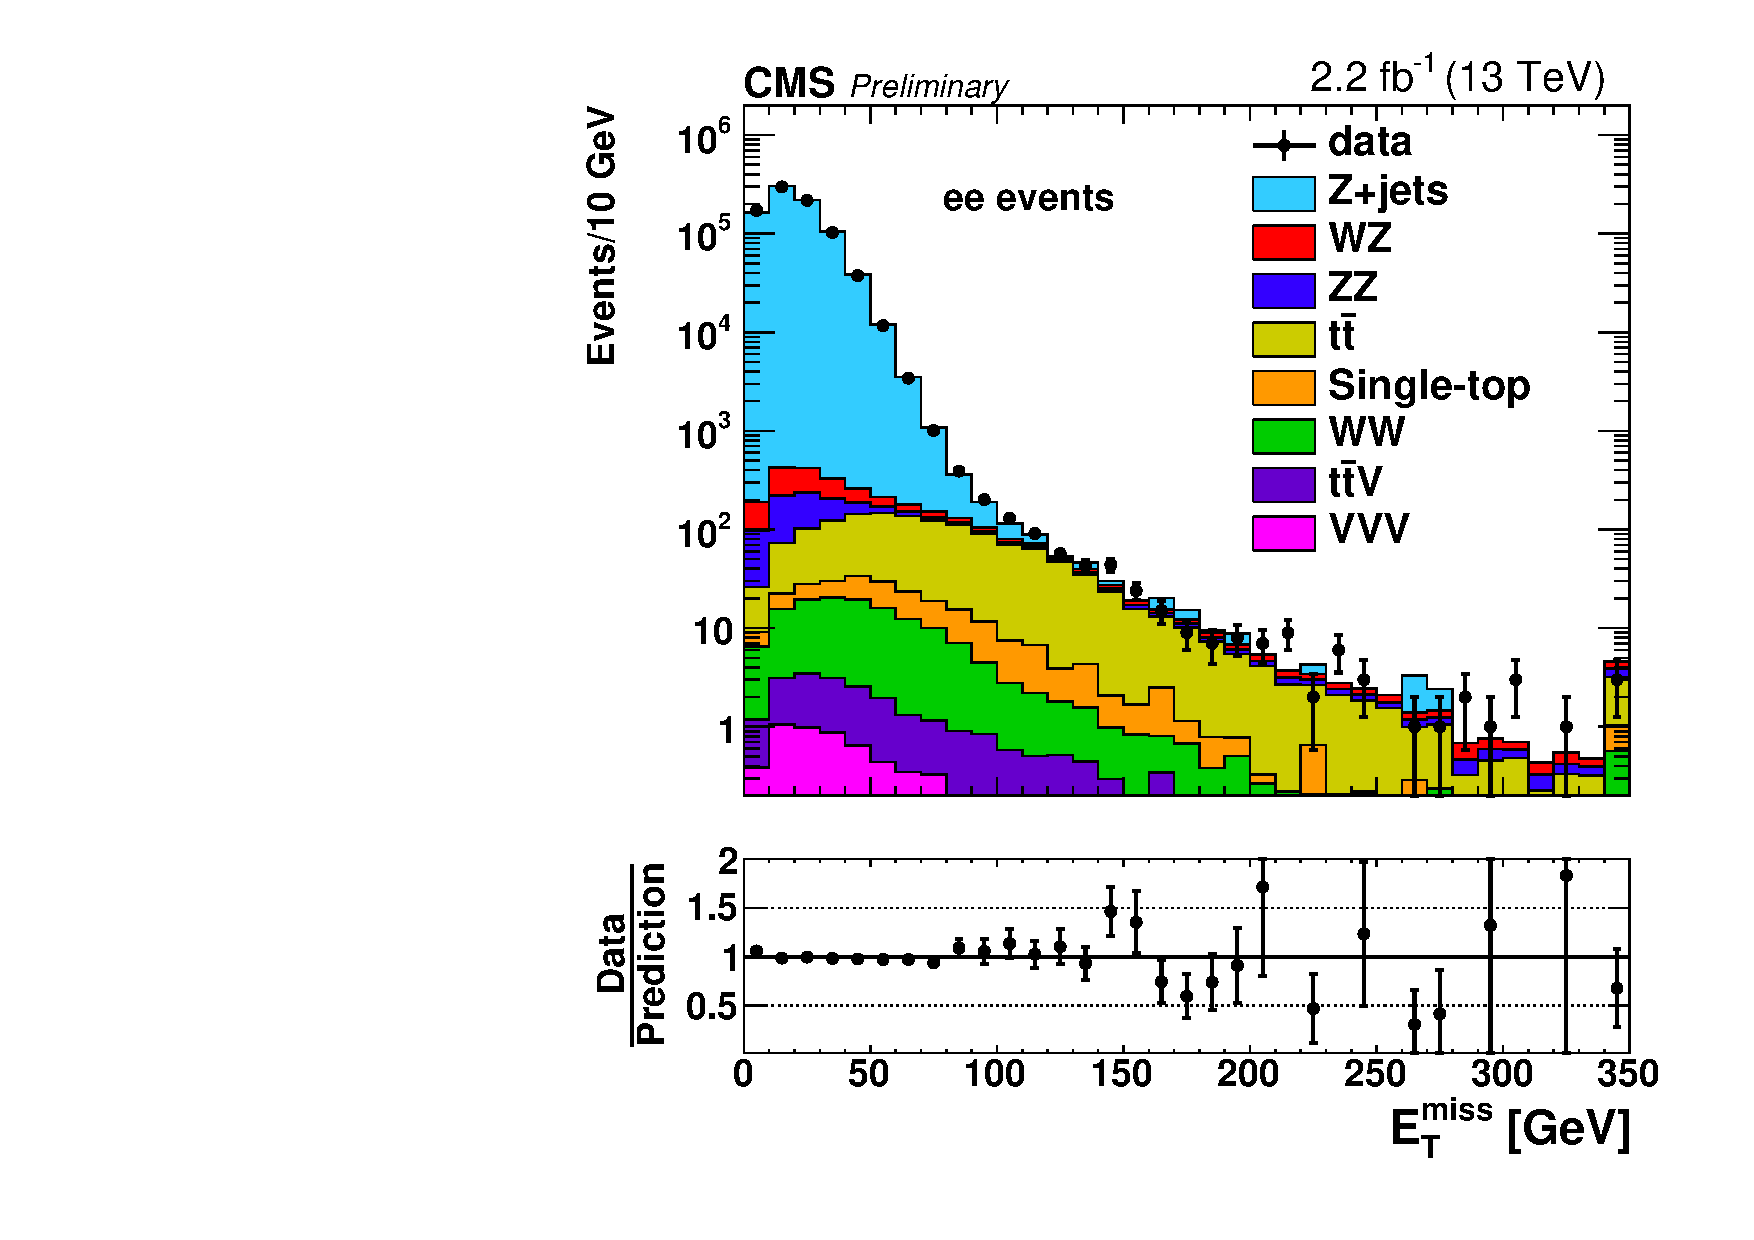
\includegraphics[width=0.4\textwidth]{MET/figs/h_met_T1CHS_pt_ee_inclusive_passtrig.pdf} &
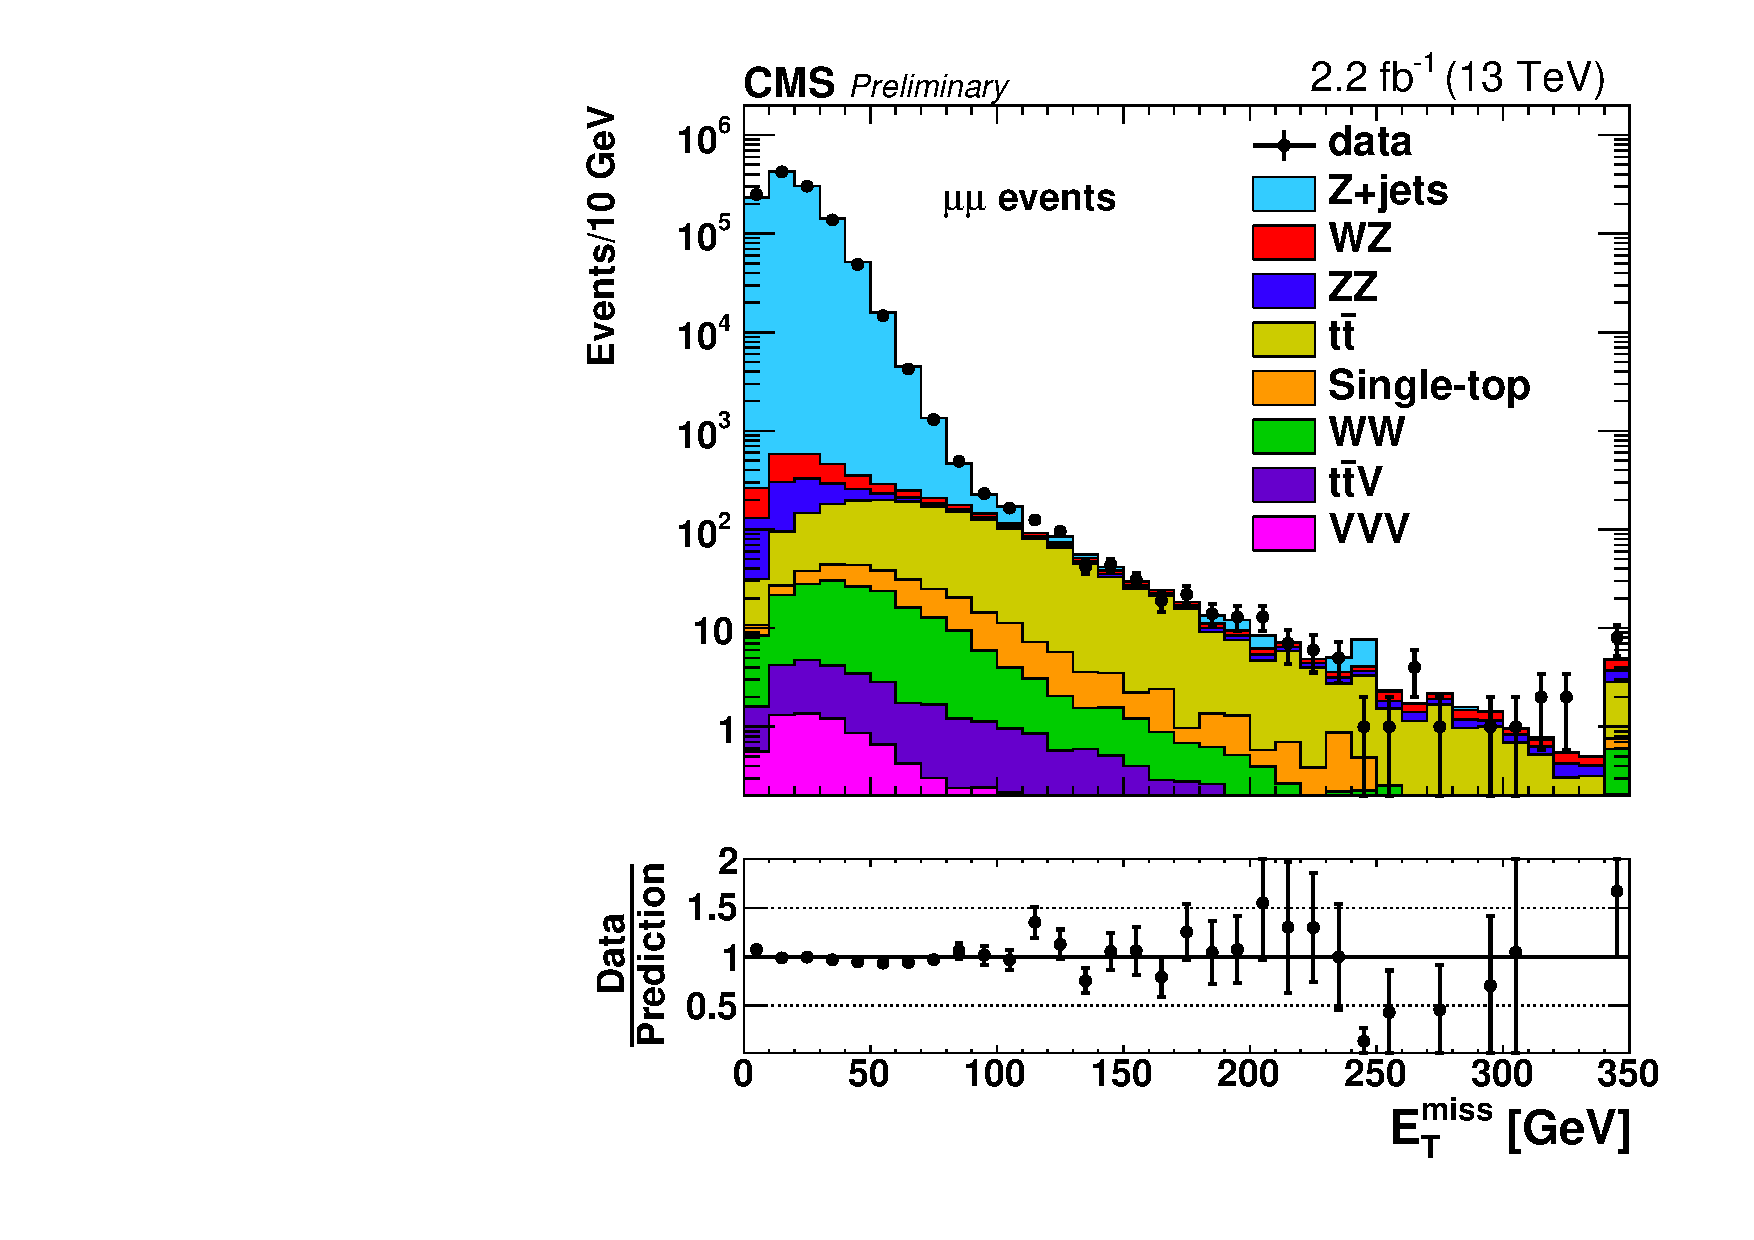
\includegraphics[width=0.4\textwidth]{MET/figs/h_met_T1CHS_pt_mm_inclusive_passtrig.pdf} \\
\end{tabular}
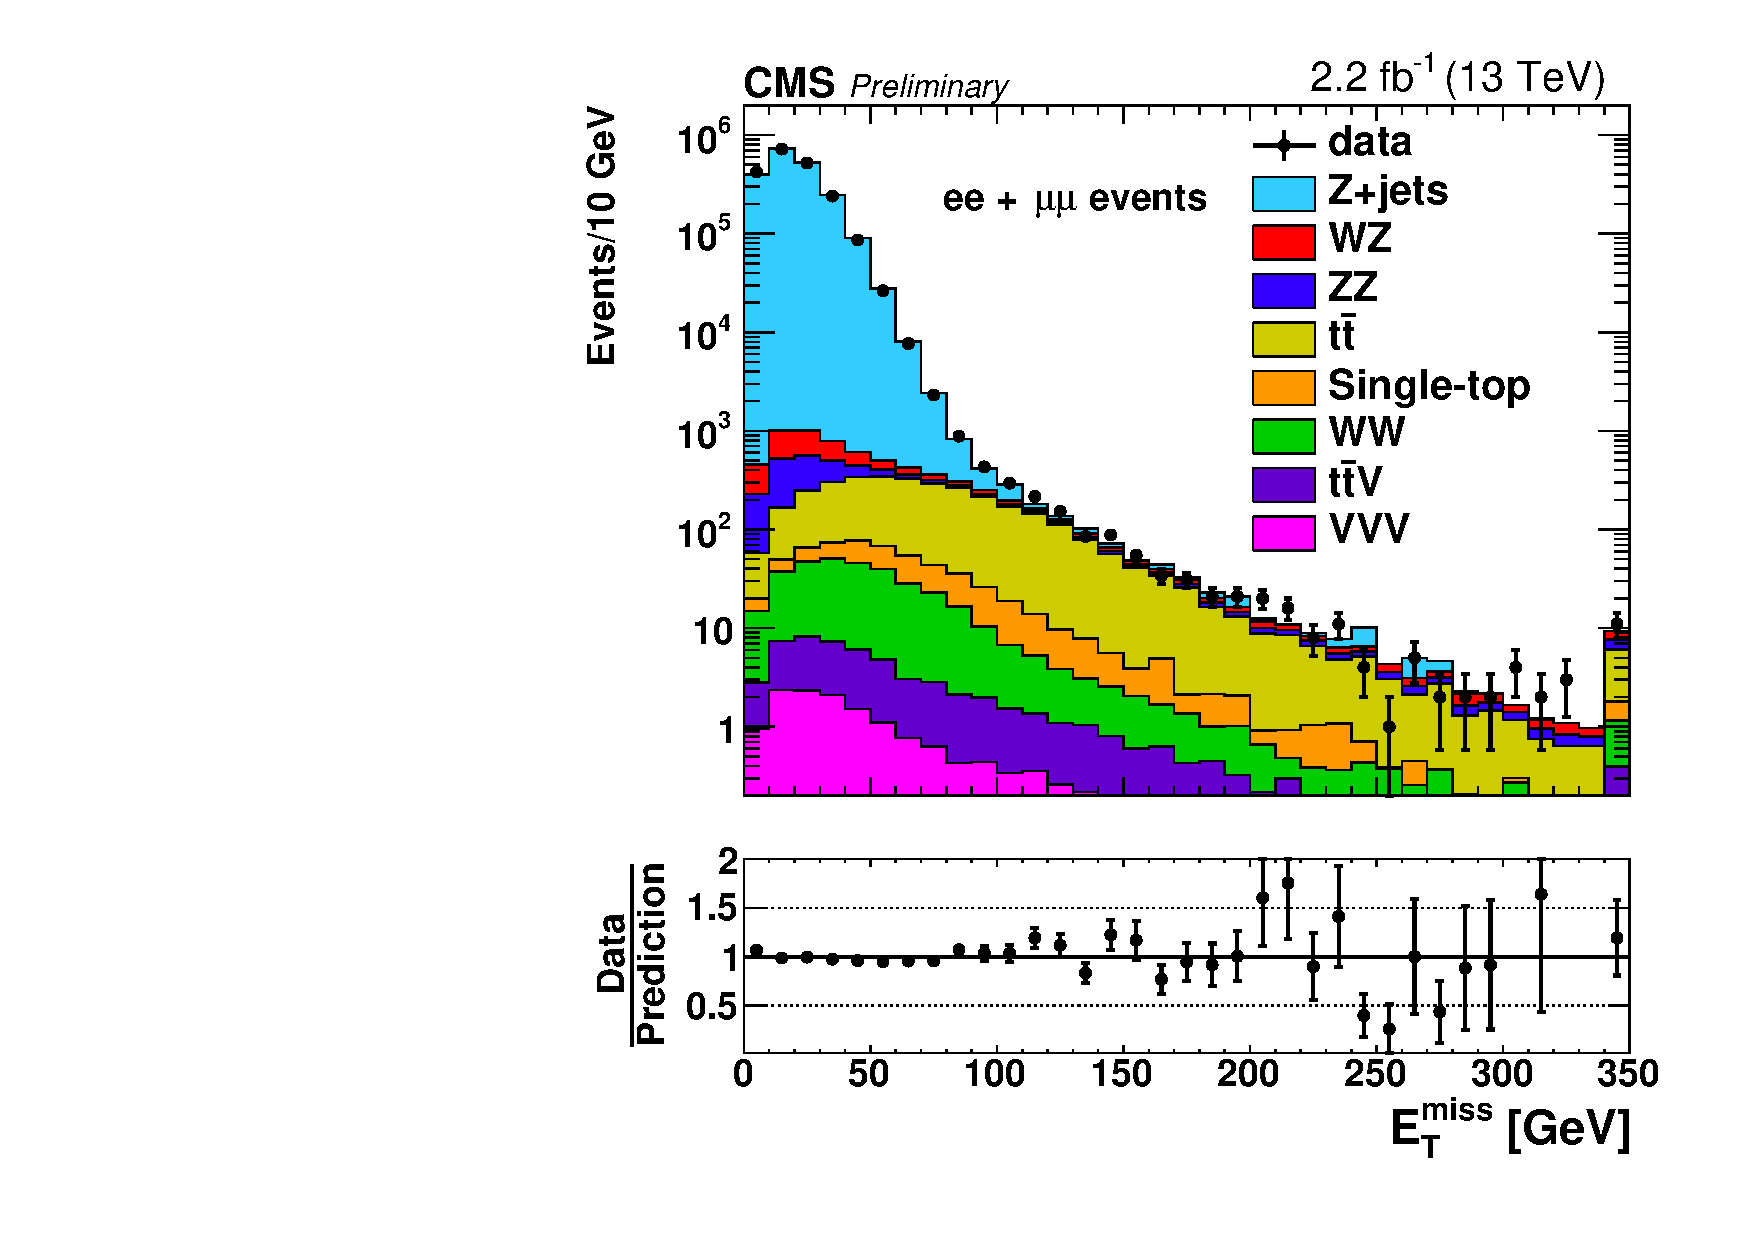
\includegraphics[width=0.6\textwidth]{MET/figs/h_met_T1CHS_pt_ll_inclusive_passtrig.pdf}
\caption{The \MET\ distribution is shown with data vs. MC for events with $Z\rightarrow\ell\ell$.
The top row shows ee events on the left and $\mu\mu$ events on the left,
and the bottom row shows ee$+\mu\mu$ events together.
\label{fig:T1MET_datavsmc}
}
\end{center}
\end{figure}

\begin{table}[htb]
\scriptsize
\begin{center}
\caption{
Definitions for the $\eta$ region chosen for each subdetector.
\label{tab:subdetector_eta}}
\begin{tabular}{l|c}

\hline
Subdetector Region     & $\eta$ cut \\
\hline
Barrel                 & $|\eta| < 1.3$ \\
Transition region      & $1.3 < |\eta| < 1.6$ \\
Endcap with tracker    & $1.6 < |\eta| < 2.4$ \\
Endcap without tracker & $2.4 < |\eta| < 3.0$ \\
HF region              & $|\eta| > 3.0$ \\
\hline
\end{tabular}
\end{center}
\end{table}


\begin{figure}[!ht]
\begin{center}
\begin{tabular}{cc}
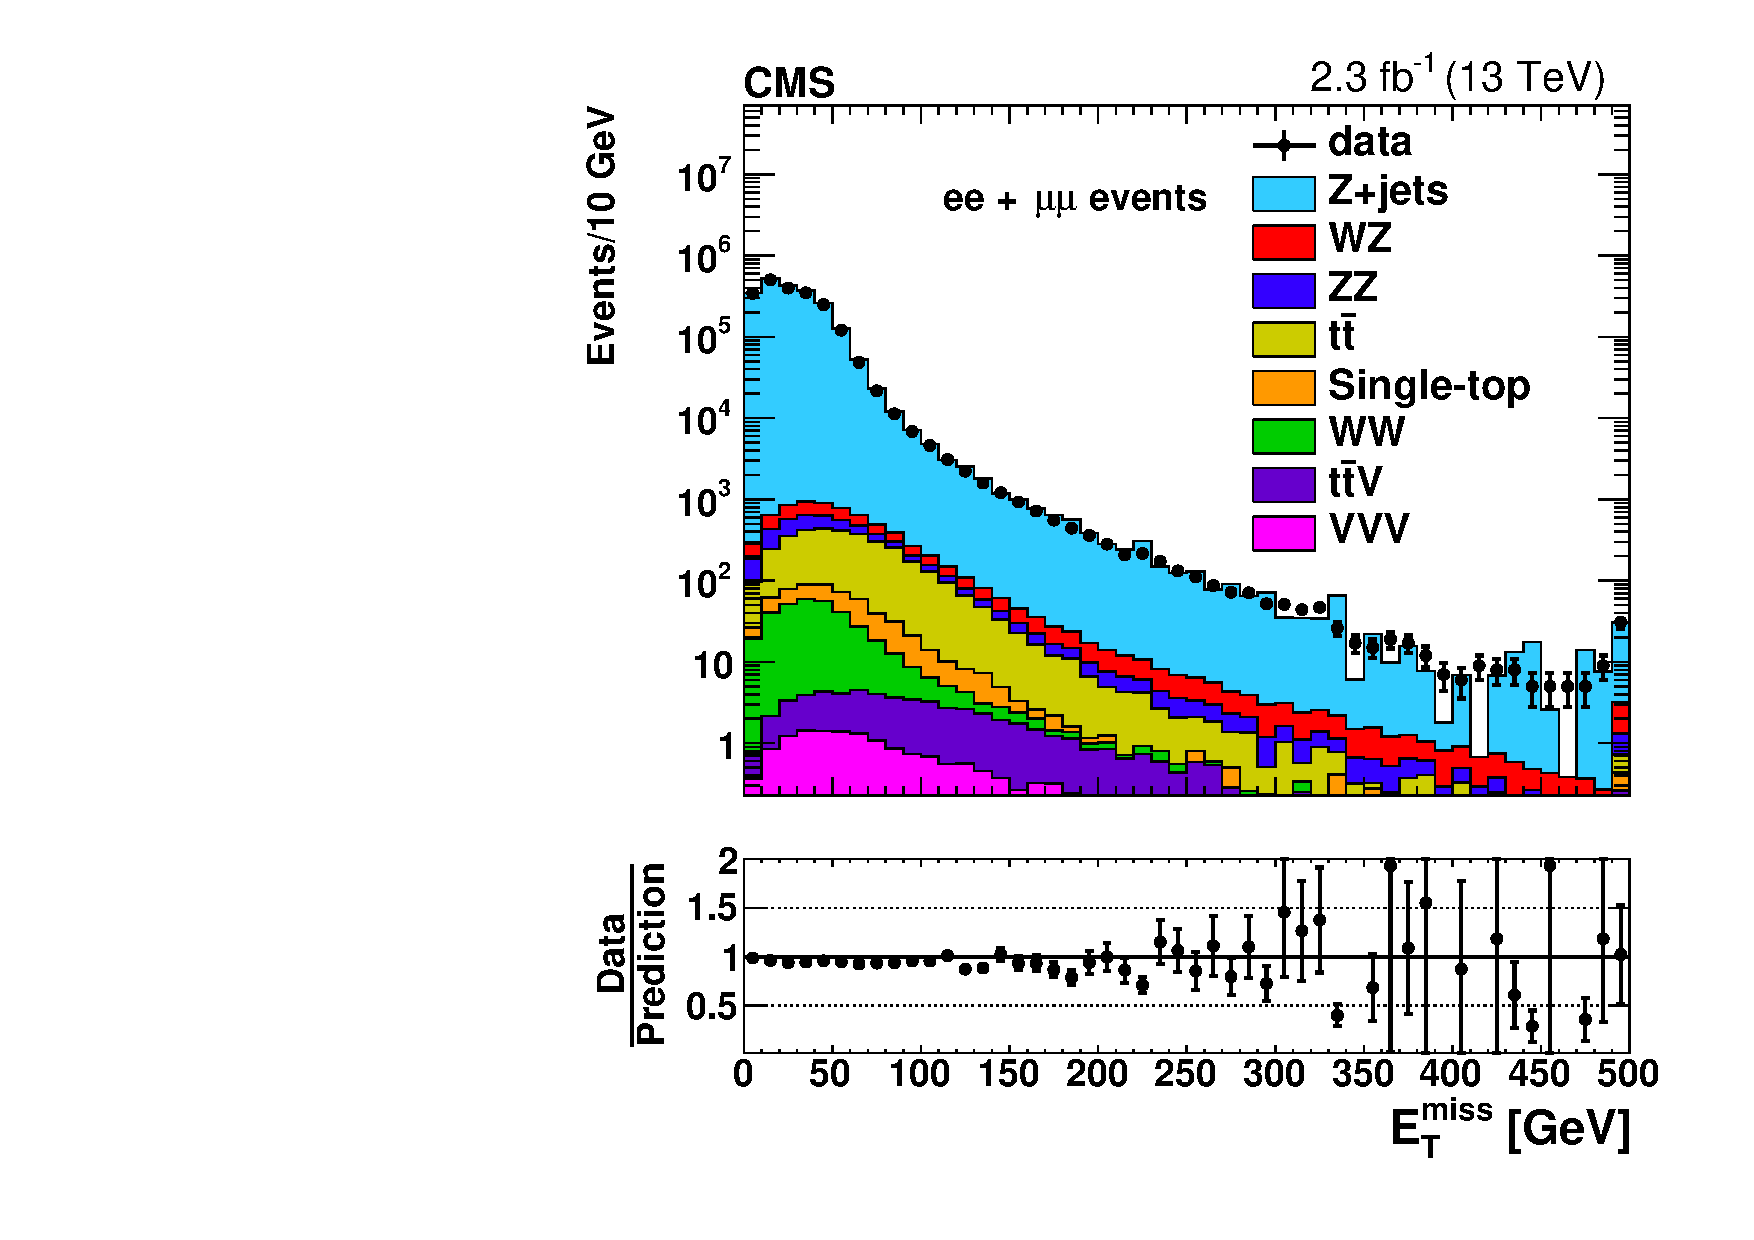
\includegraphics[width=0.4\textwidth]{MET/figs/h_met_chpfcands_0013_pt_ll_signalregion_inclusive_passtrig.pdf} &
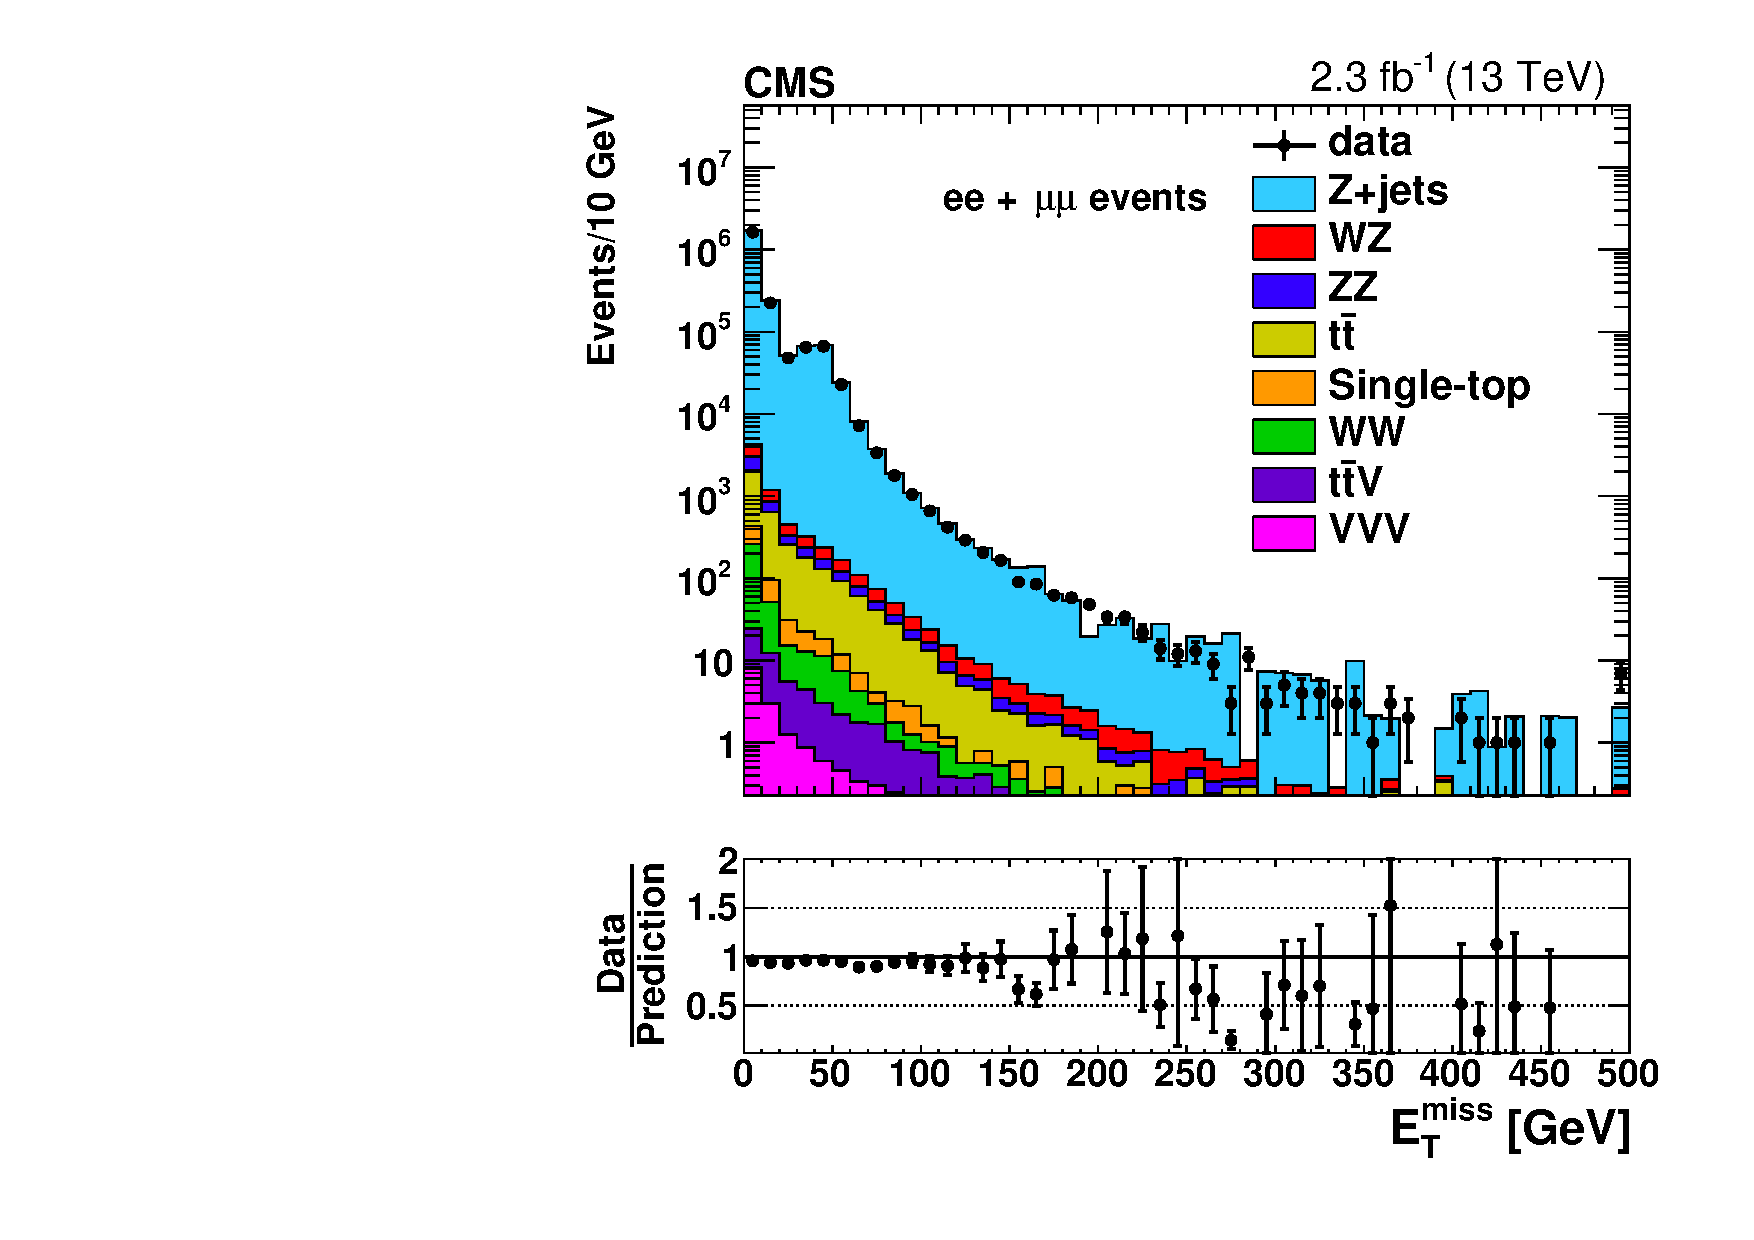
\includegraphics[width=0.4\textwidth]{MET/figs/h_met_chpfcands_1316_pt_ll_signalregion_inclusive_passtrig.pdf} \\
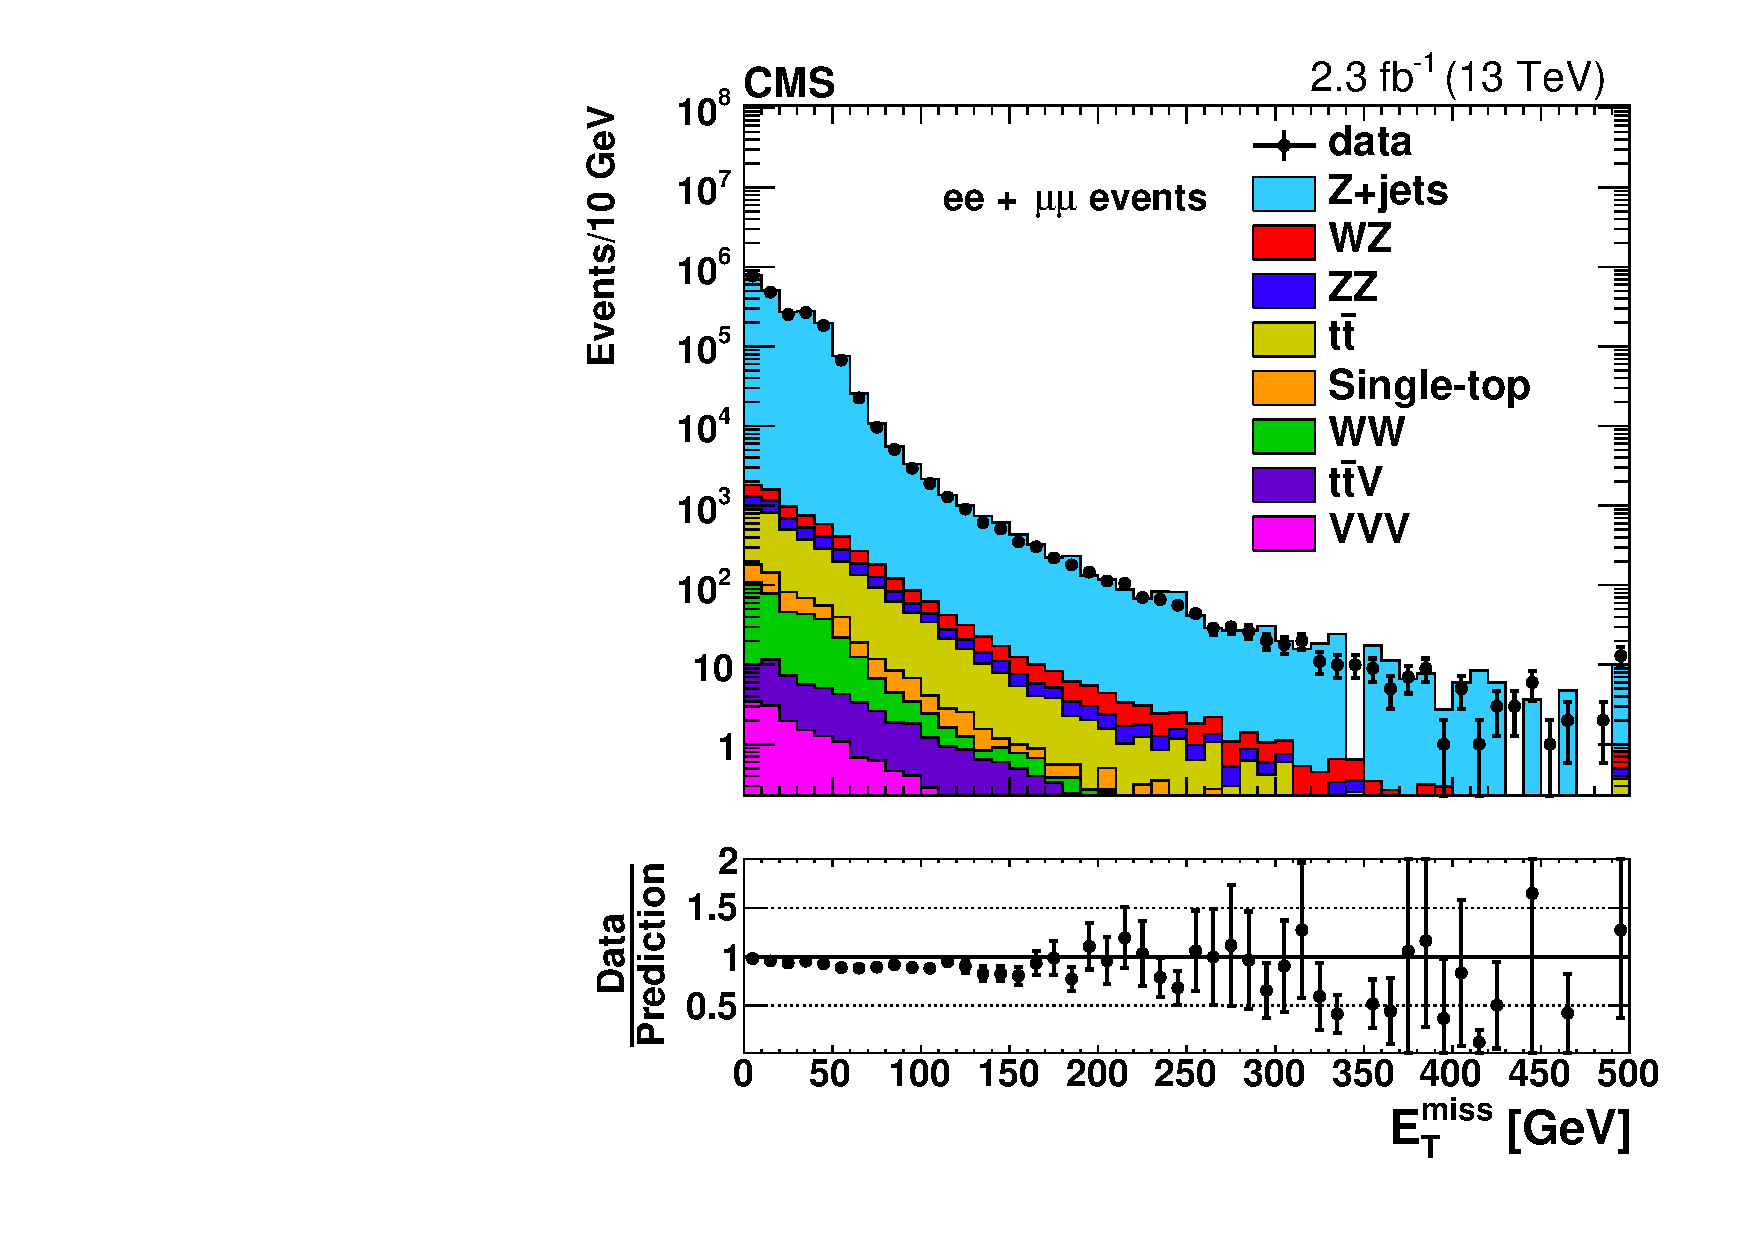
\includegraphics[width=0.4\textwidth]{MET/figs/h_met_chpfcands_1624_pt_ll_signalregion_inclusive_passtrig.pdf} &
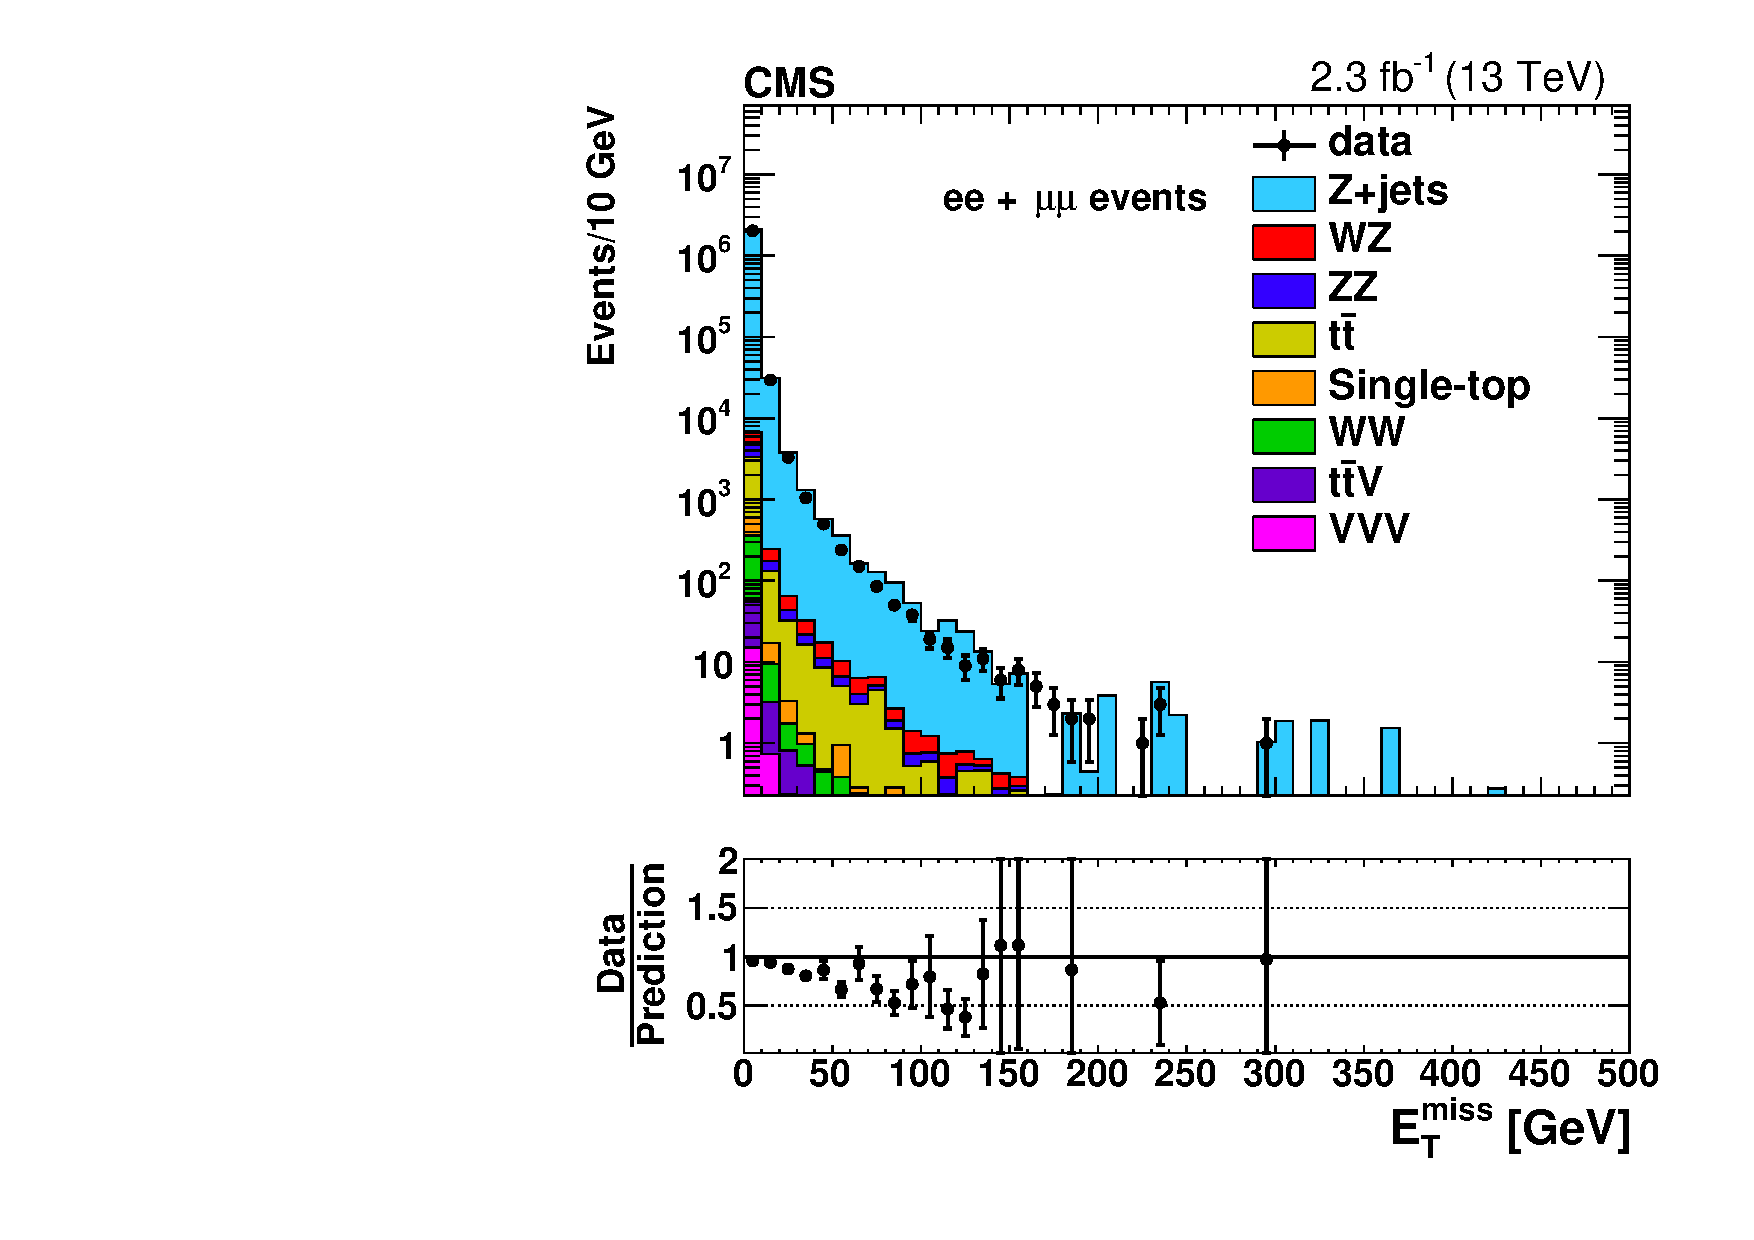
\includegraphics[width=0.4\textwidth]{MET/figs/h_met_chpfcands_2430_pt_ll_signalregion_inclusive_passtrig.pdf} \\
\end{tabular}
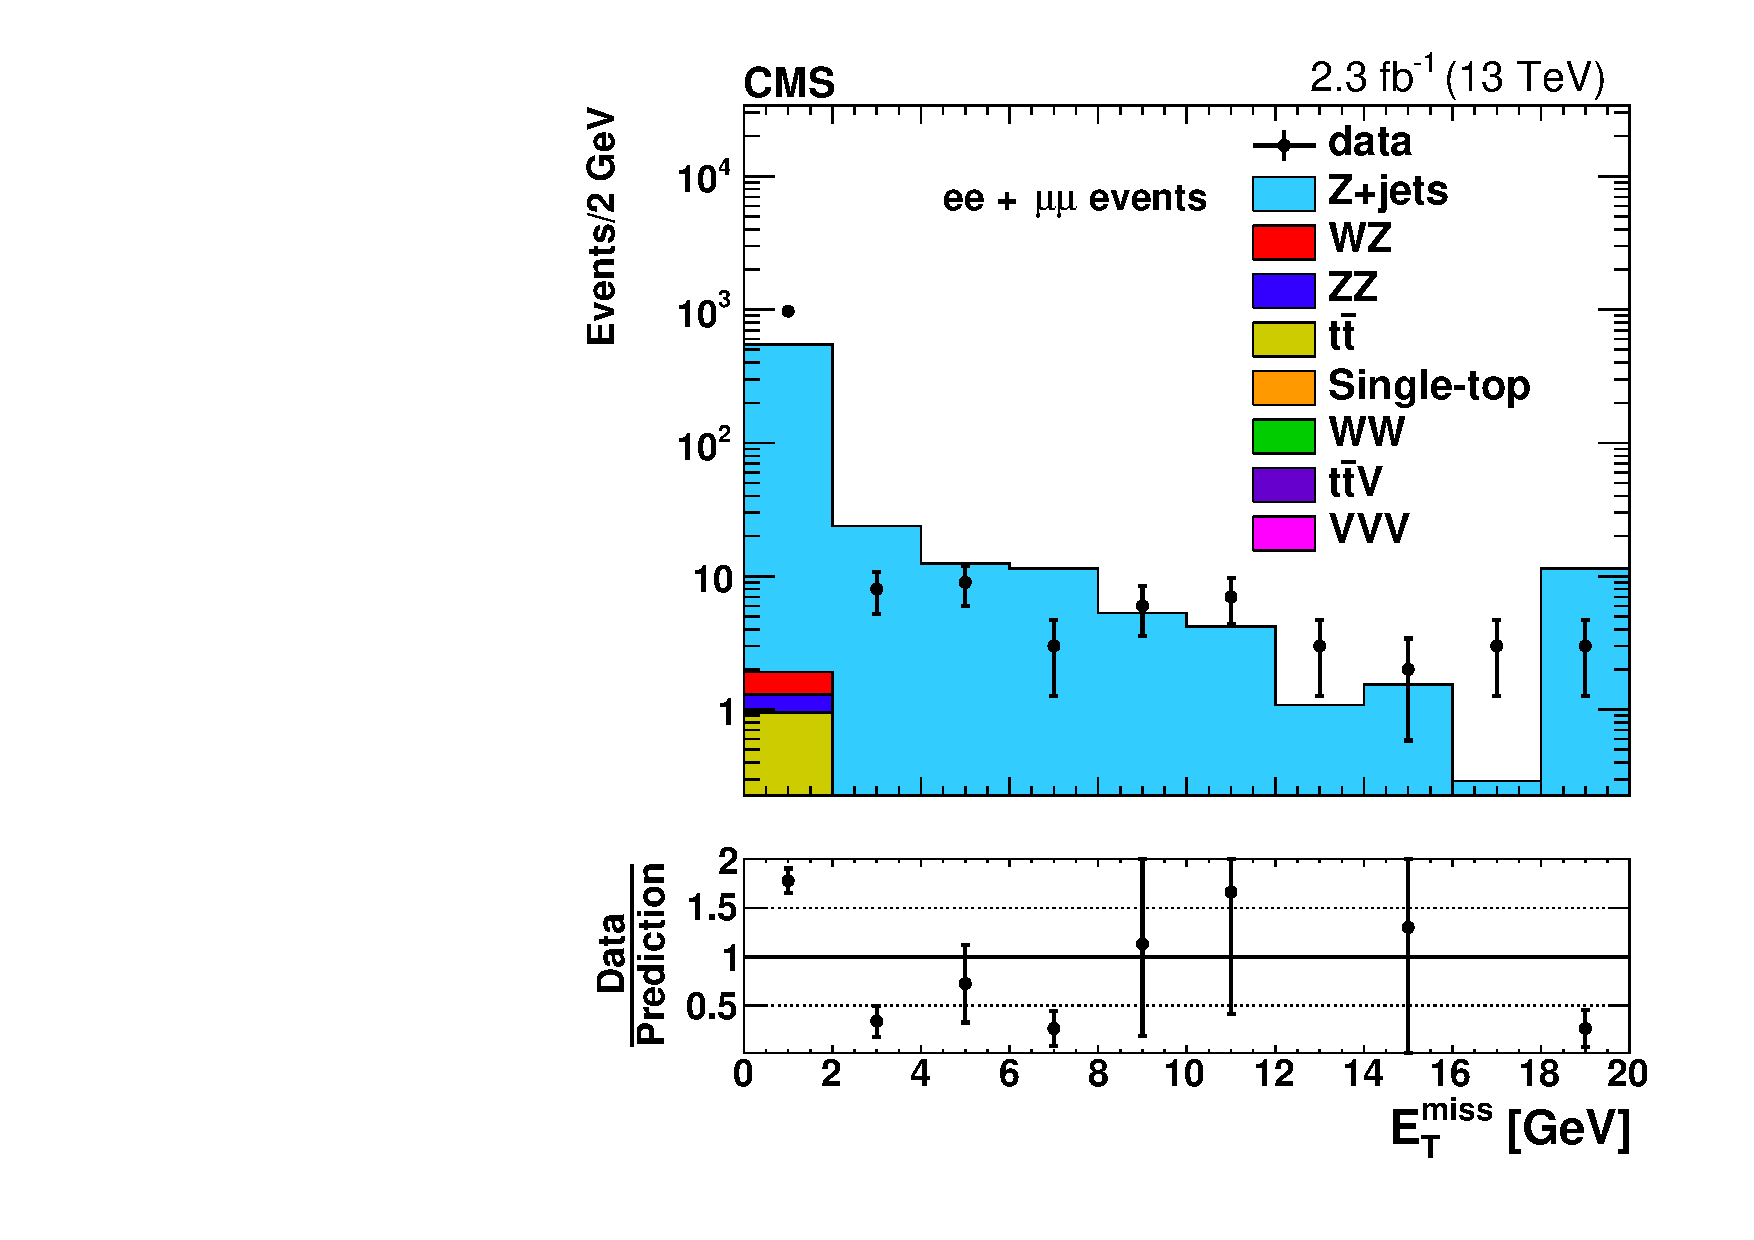
\includegraphics[width=0.4\textwidth]{MET/figs/h_met_chpfcands_30in_pt_ll_signalregion_inclusive_passtrig.pdf} 
\caption{The \MET\ distribution is shown for charged PF candidates only.
The top row shows the barrel region on the left and transition region between the barrel and endcap on the right,
the second row shows the endcap region including the tracker on the left and endcap region excluding the tracker on the right
and the bottom row shows the HF region only.
\label{fig:chpfcands}
}
\end{center}
\end{figure}

\begin{figure}[!ht]
\begin{center}
\begin{tabular}{cc}
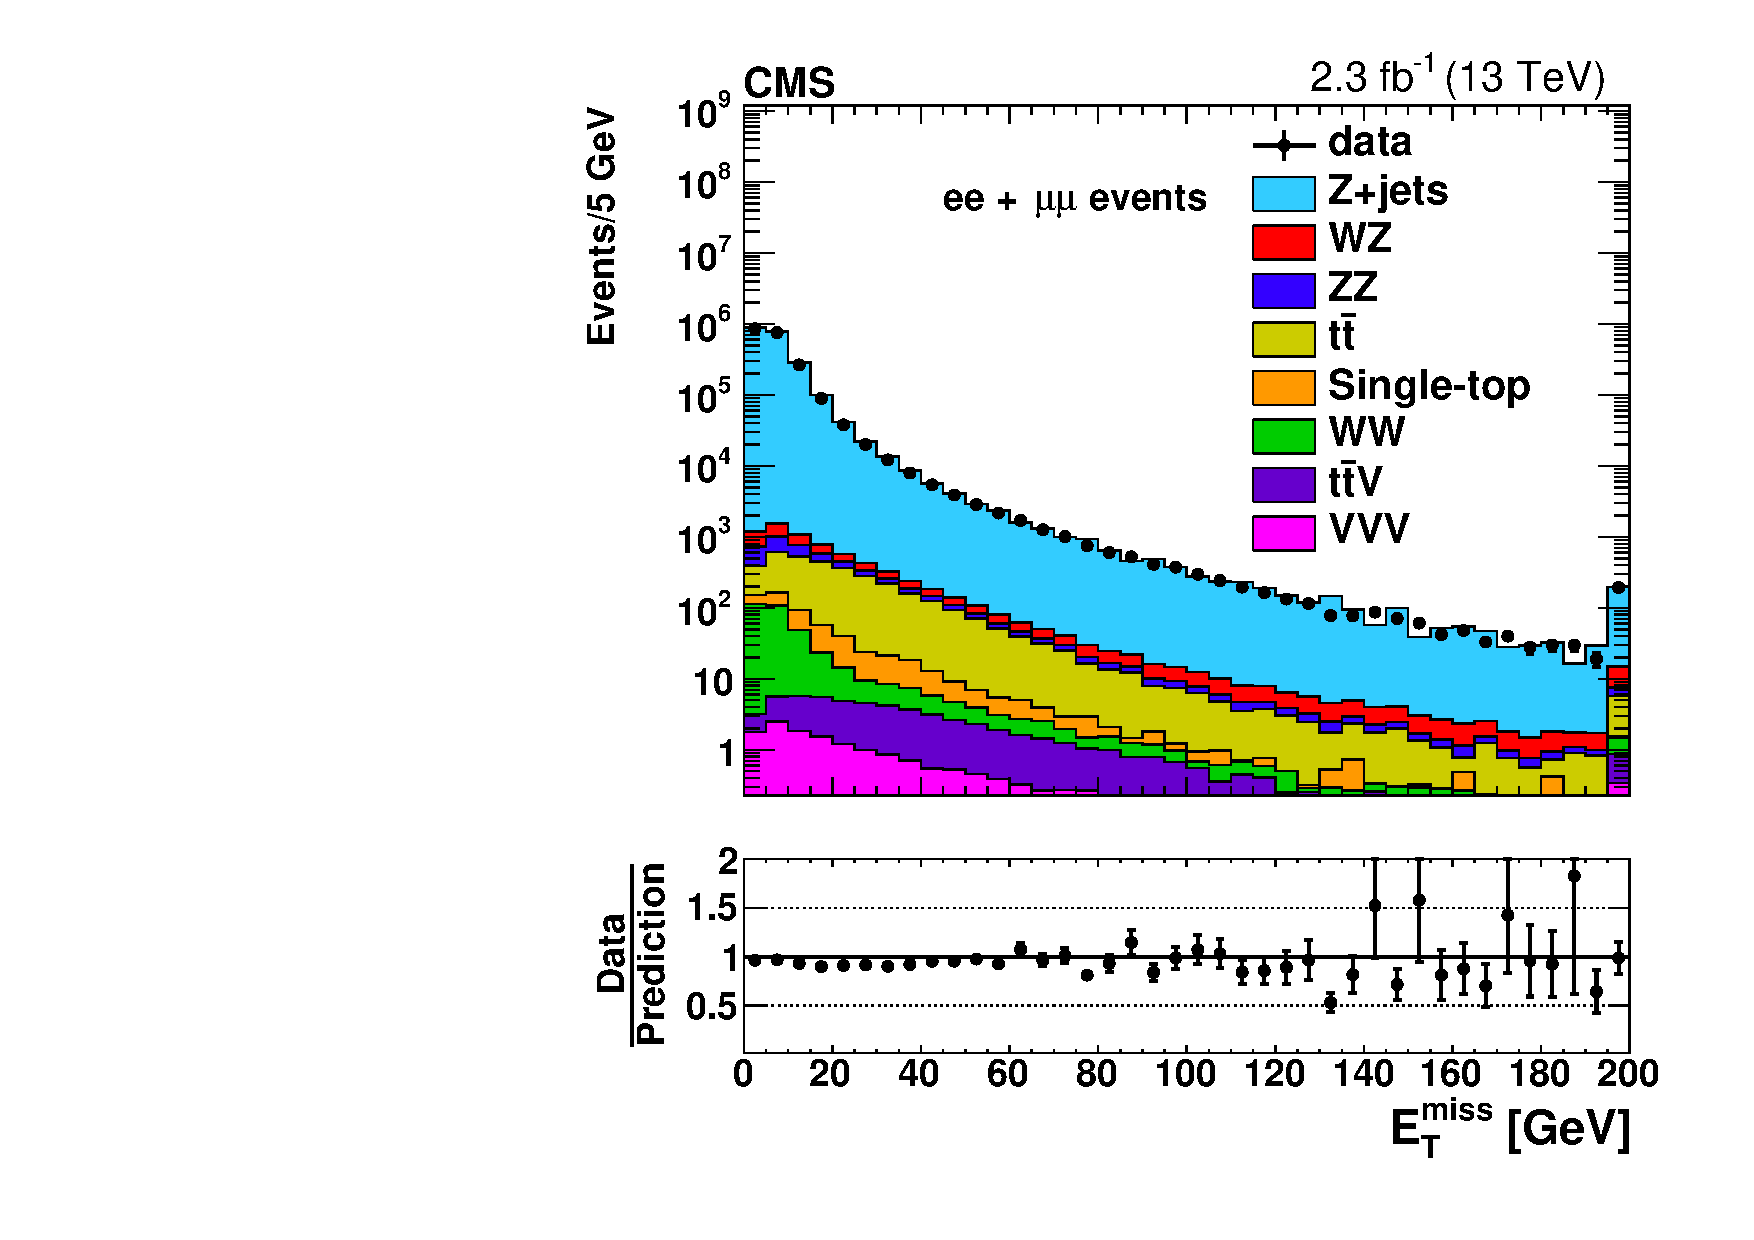
\includegraphics[width=0.4\textwidth]{MET/figs/h_met_phpfcands_0013_pt_ll_signalregion_inclusive_passtrig.pdf} &
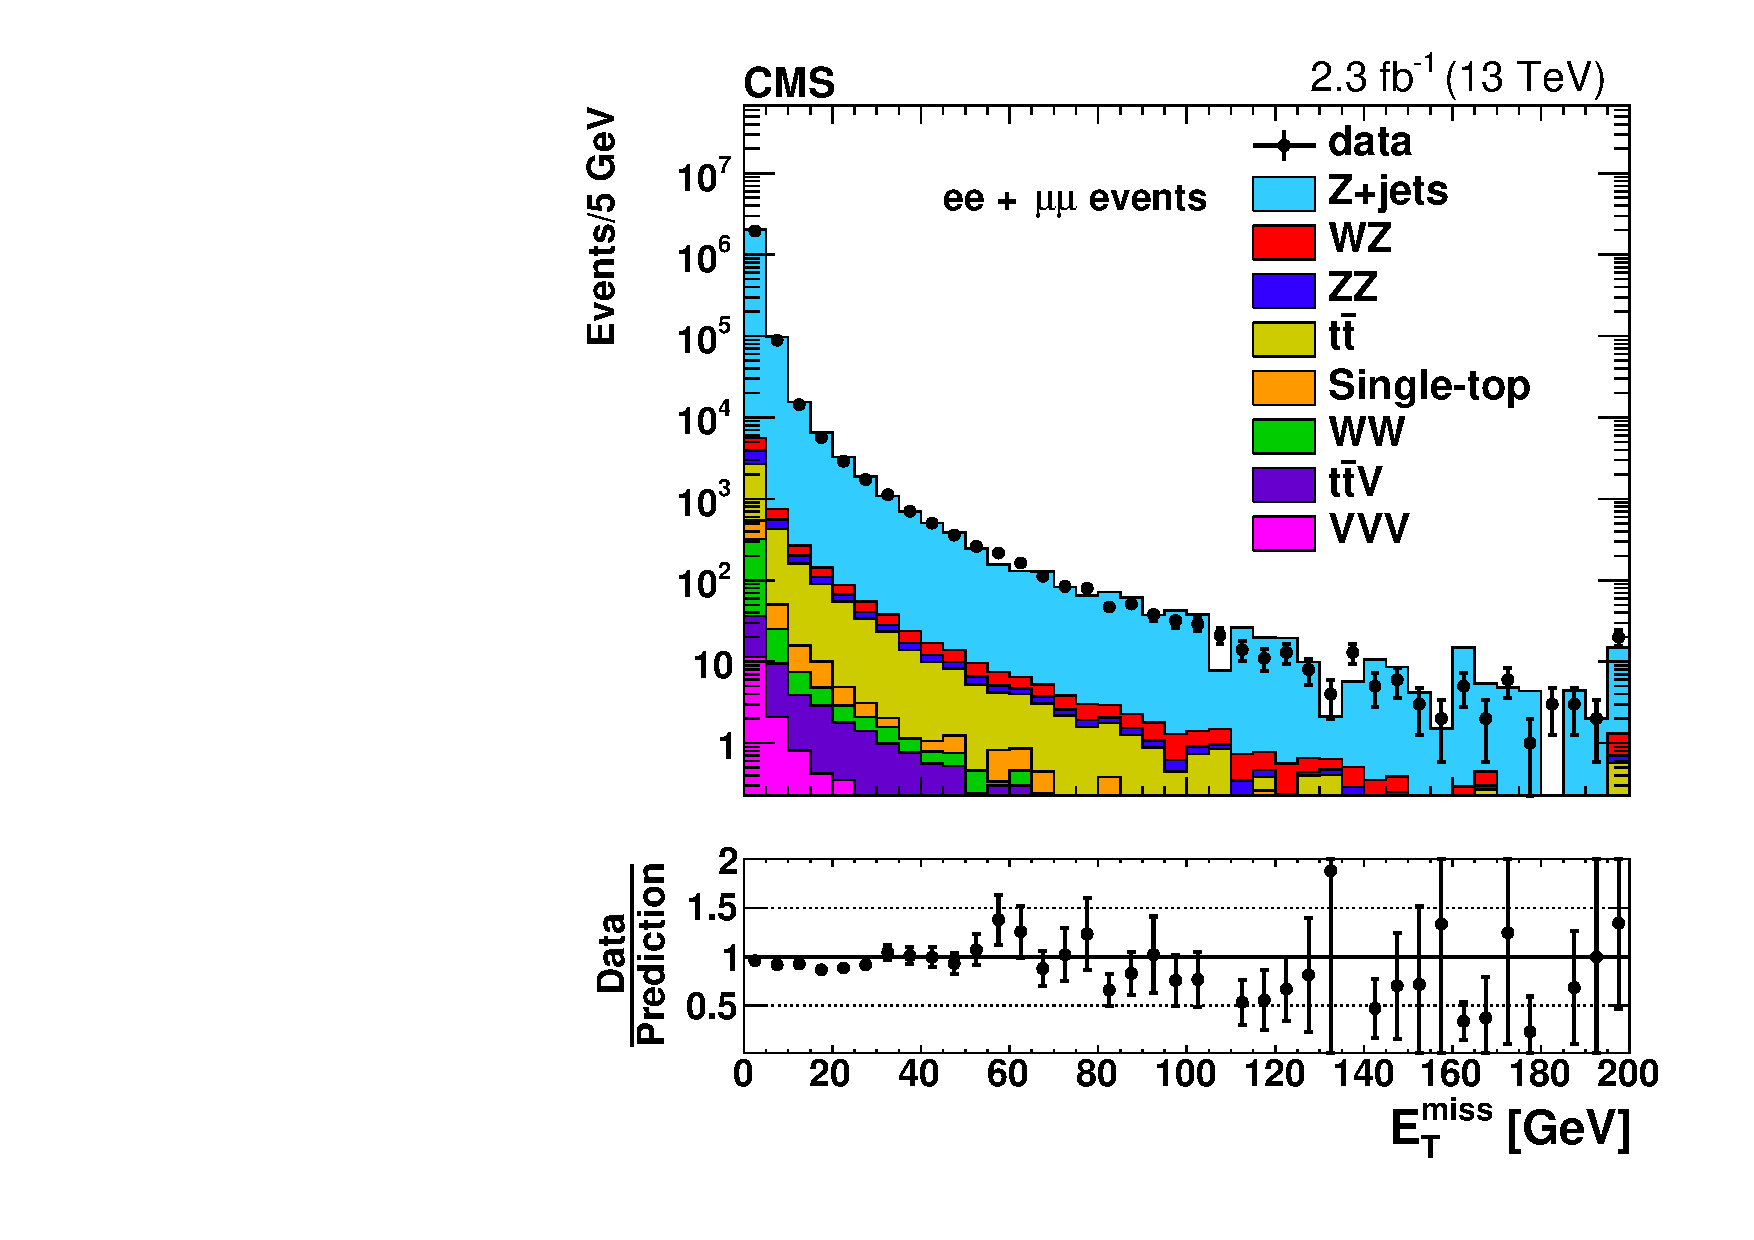
\includegraphics[width=0.4\textwidth]{MET/figs/h_met_phpfcands_1316_pt_ll_signalregion_inclusive_passtrig.pdf} \\
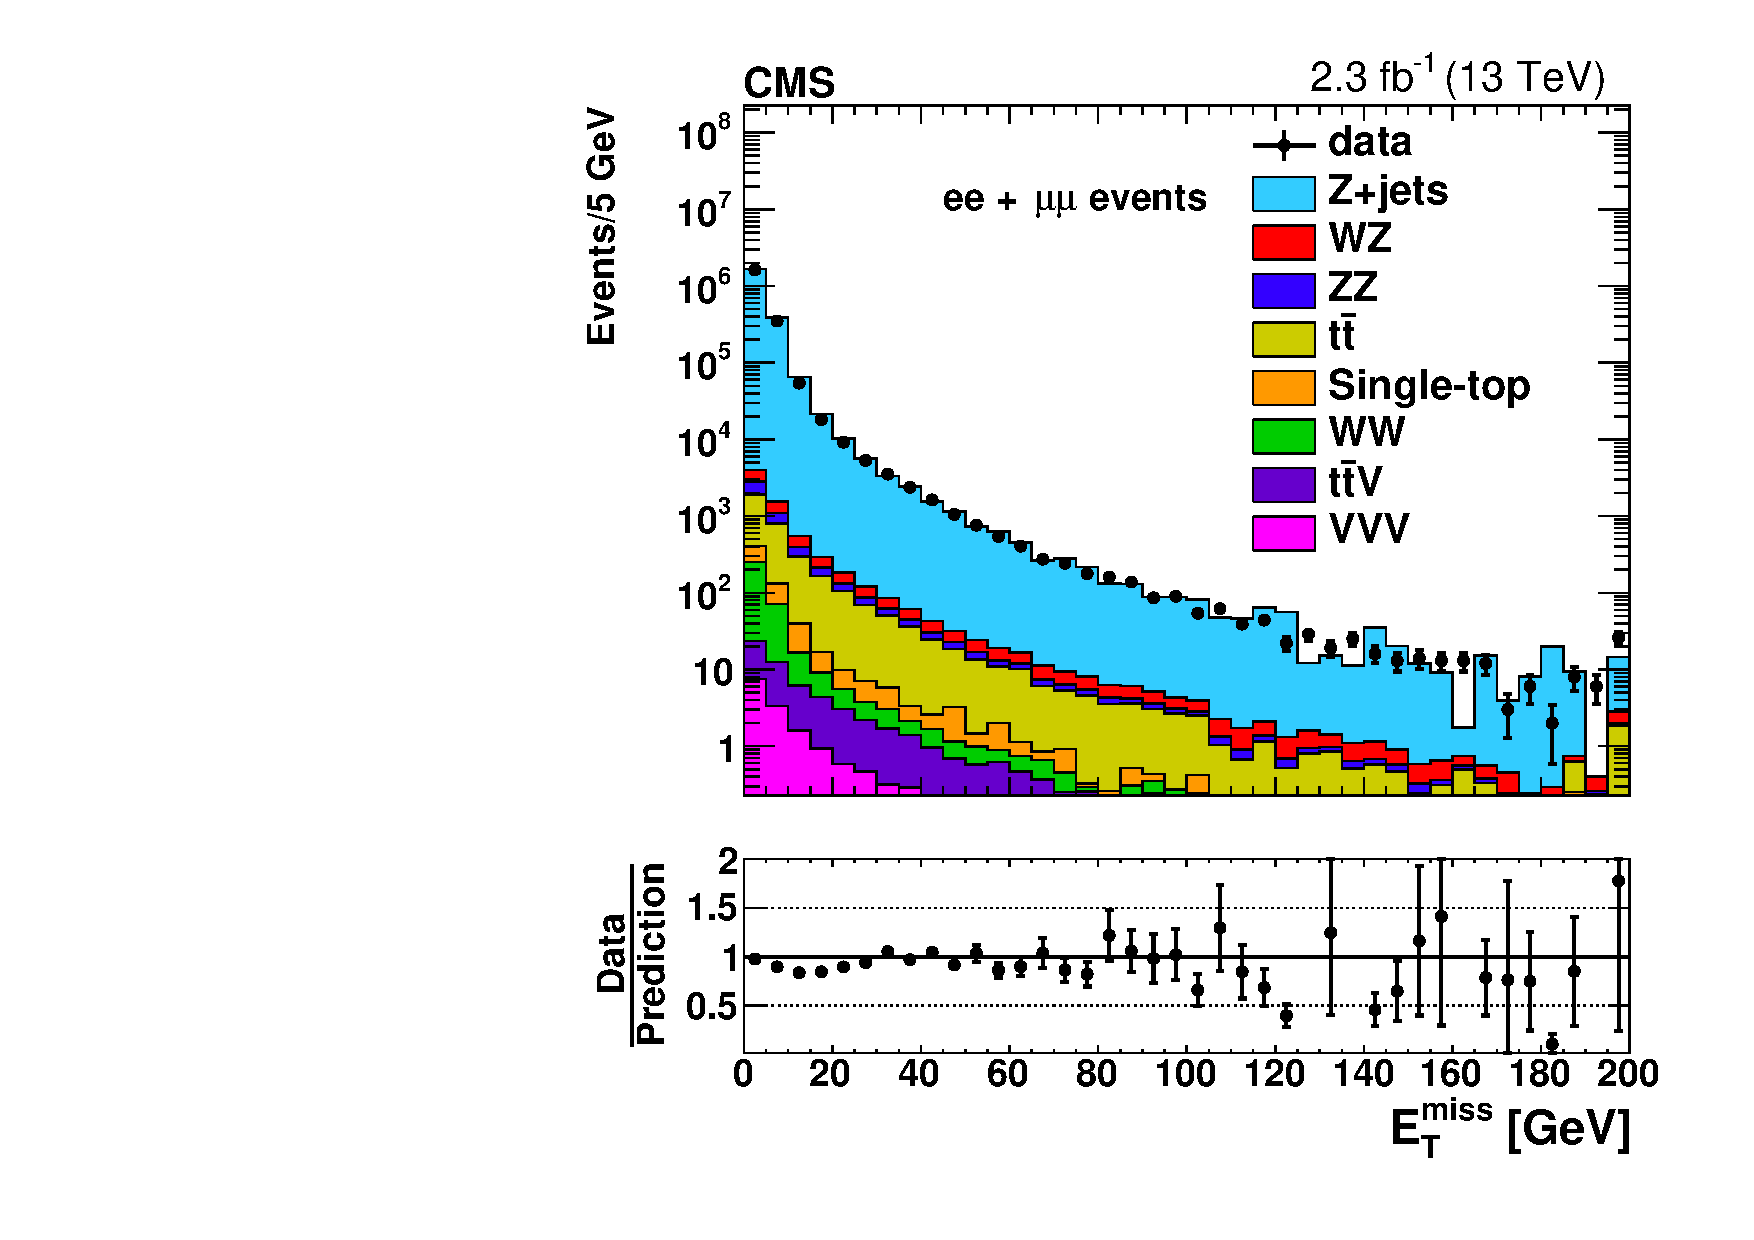
\includegraphics[width=0.4\textwidth]{MET/figs/h_met_phpfcands_1624_pt_ll_signalregion_inclusive_passtrig.pdf} &
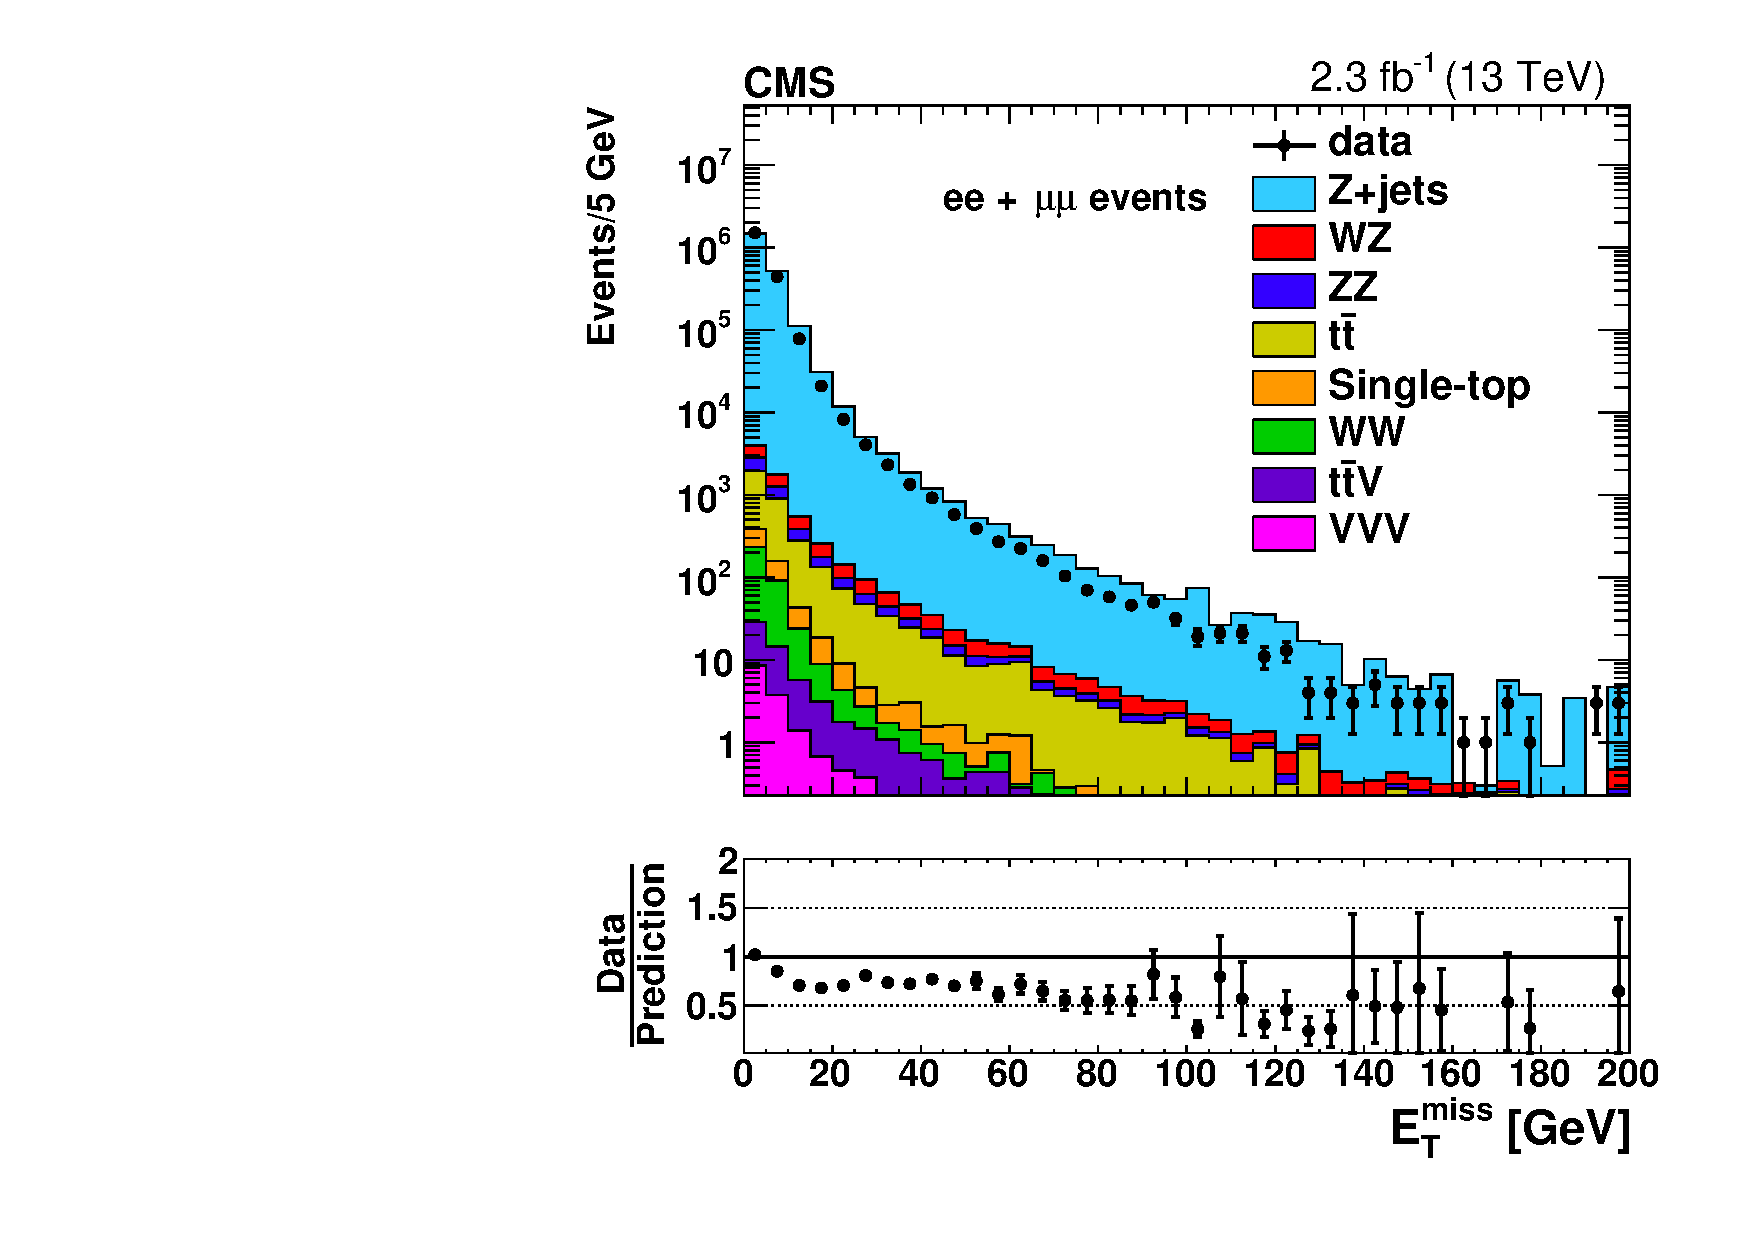
\includegraphics[width=0.4\textwidth]{MET/figs/h_met_phpfcands_2430_pt_ll_signalregion_inclusive_passtrig.pdf} \\
\end{tabular}
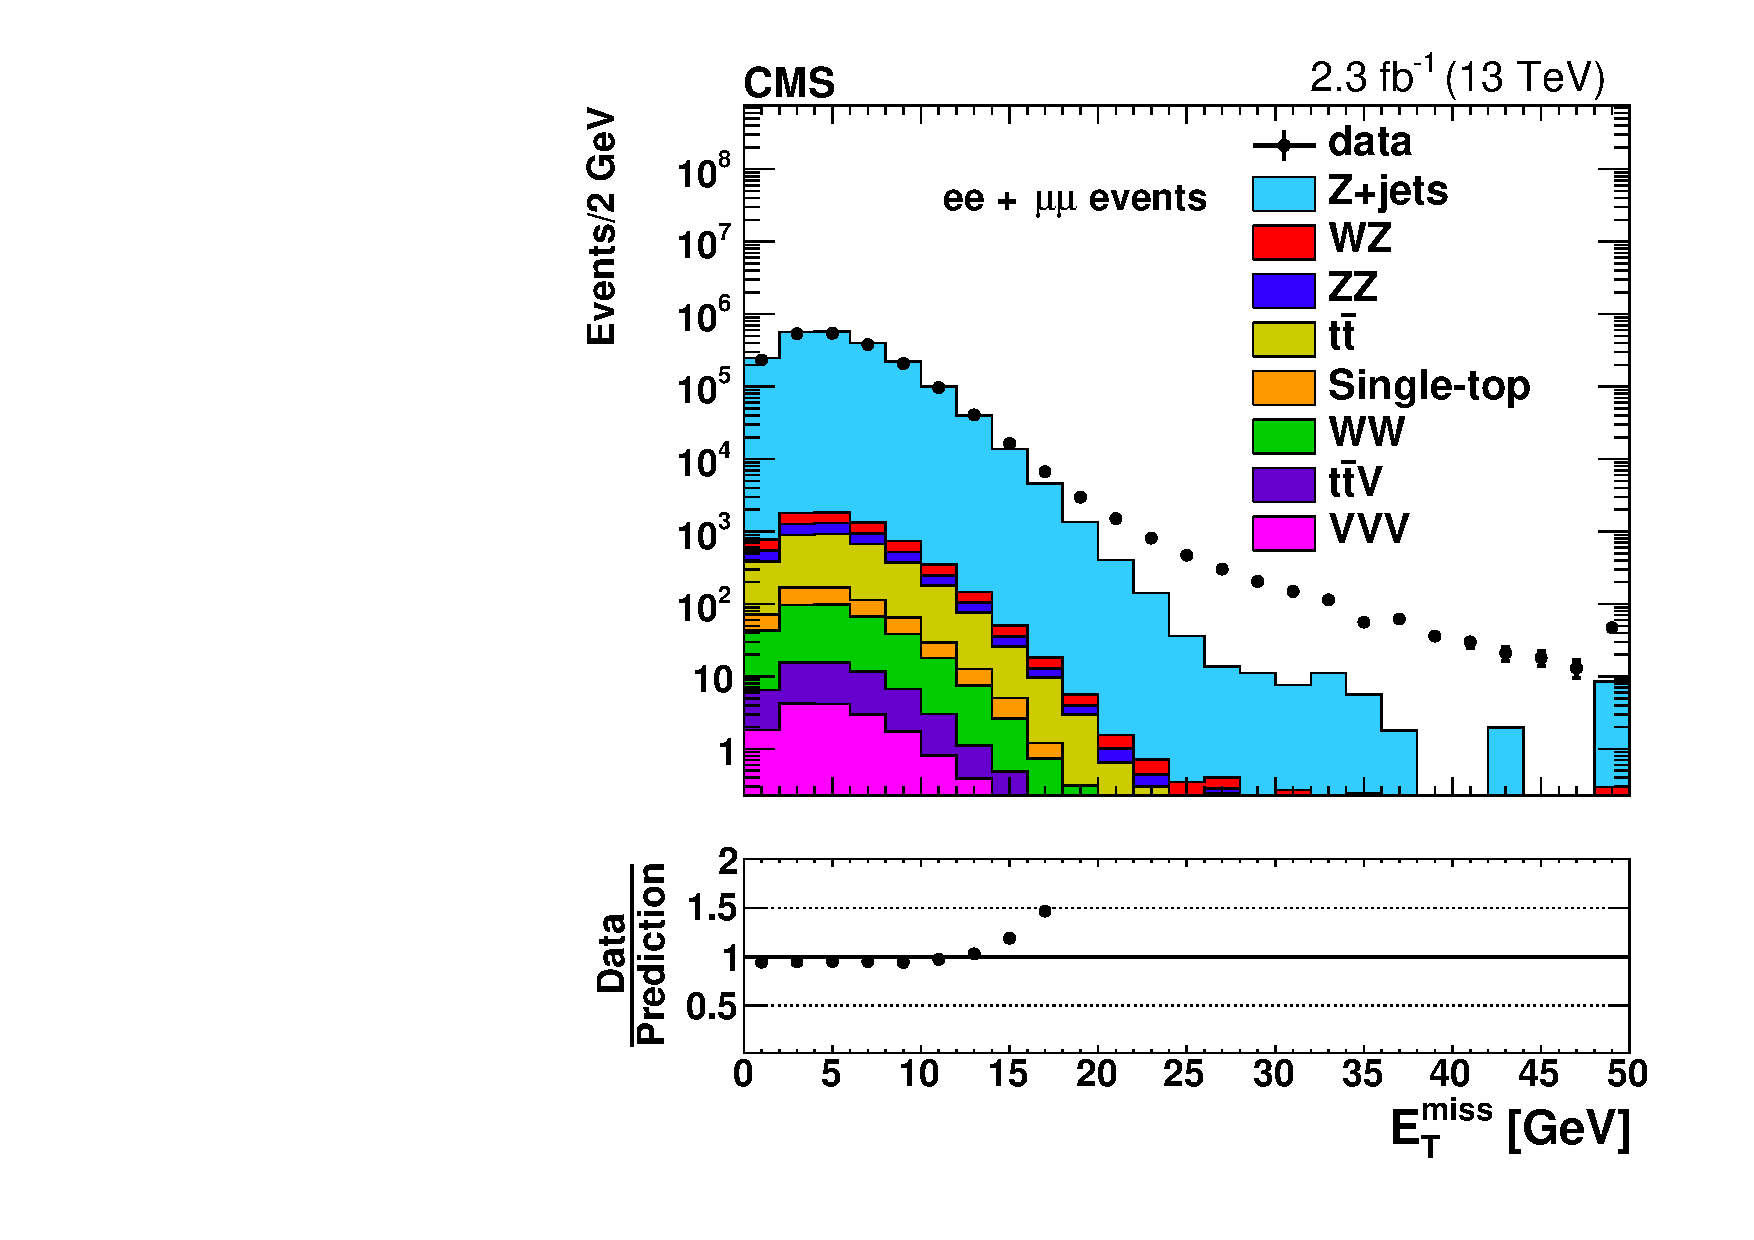
\includegraphics[width=0.4\textwidth]{MET/figs/h_met_phpfcands_30in_pt_ll_signalregion_inclusive_passtrig.pdf} 
\caption{The \MET\ distribution is shown for neutral electromagnetic PF candidates only.
The top row shows the barrel region on the left and transition region between the barrel and endcap on the right,
the second row shows the endcap region including the tracker on the left and endcap region excluding the tracker on the right
and the bottom row shows the HF region only.
\label{fig:phpfcands}
}
\end{center}
\end{figure}

\begin{figure}[!ht]
\begin{center}
\begin{tabular}{cc}
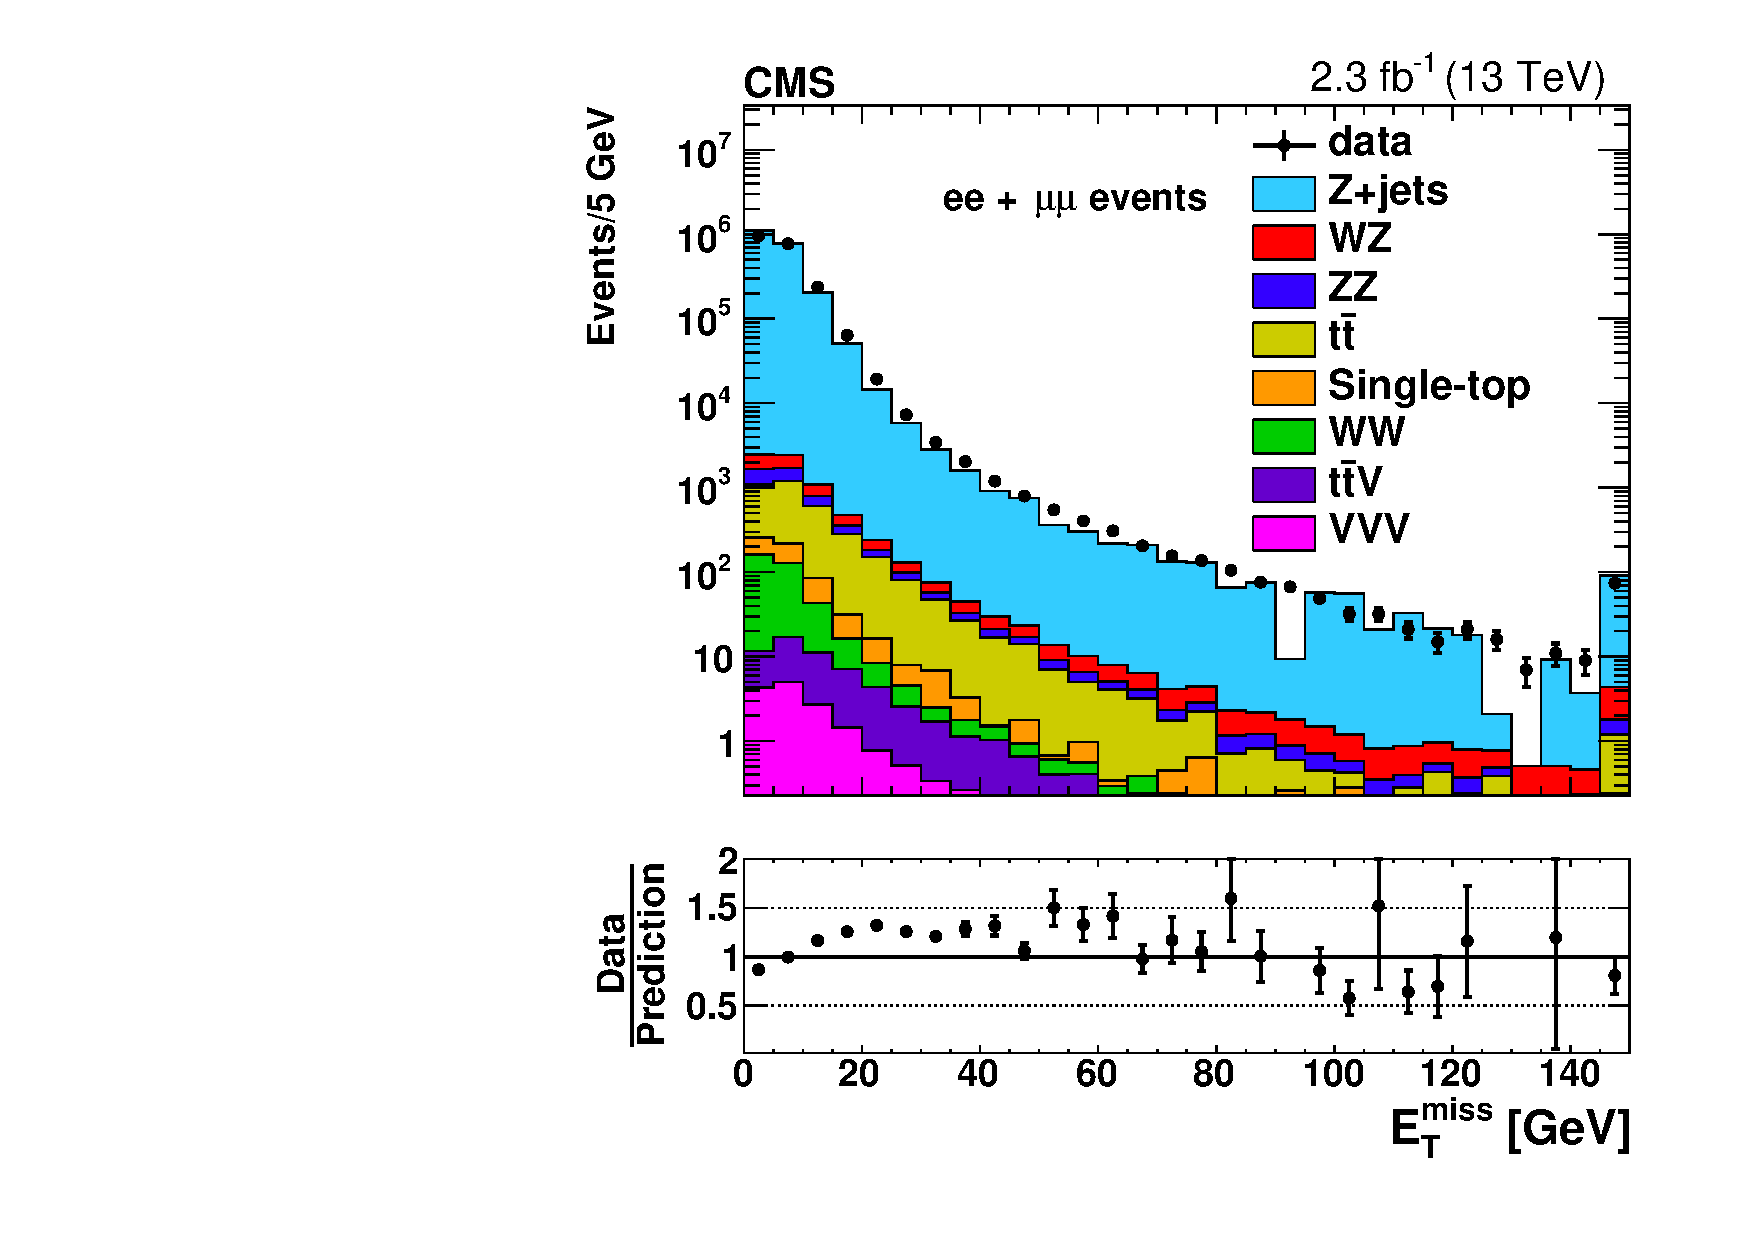
\includegraphics[width=0.4\textwidth]{MET/figs/h_met_nupfcands_0013_pt_ll_signalregion_inclusive_passtrig.pdf} &
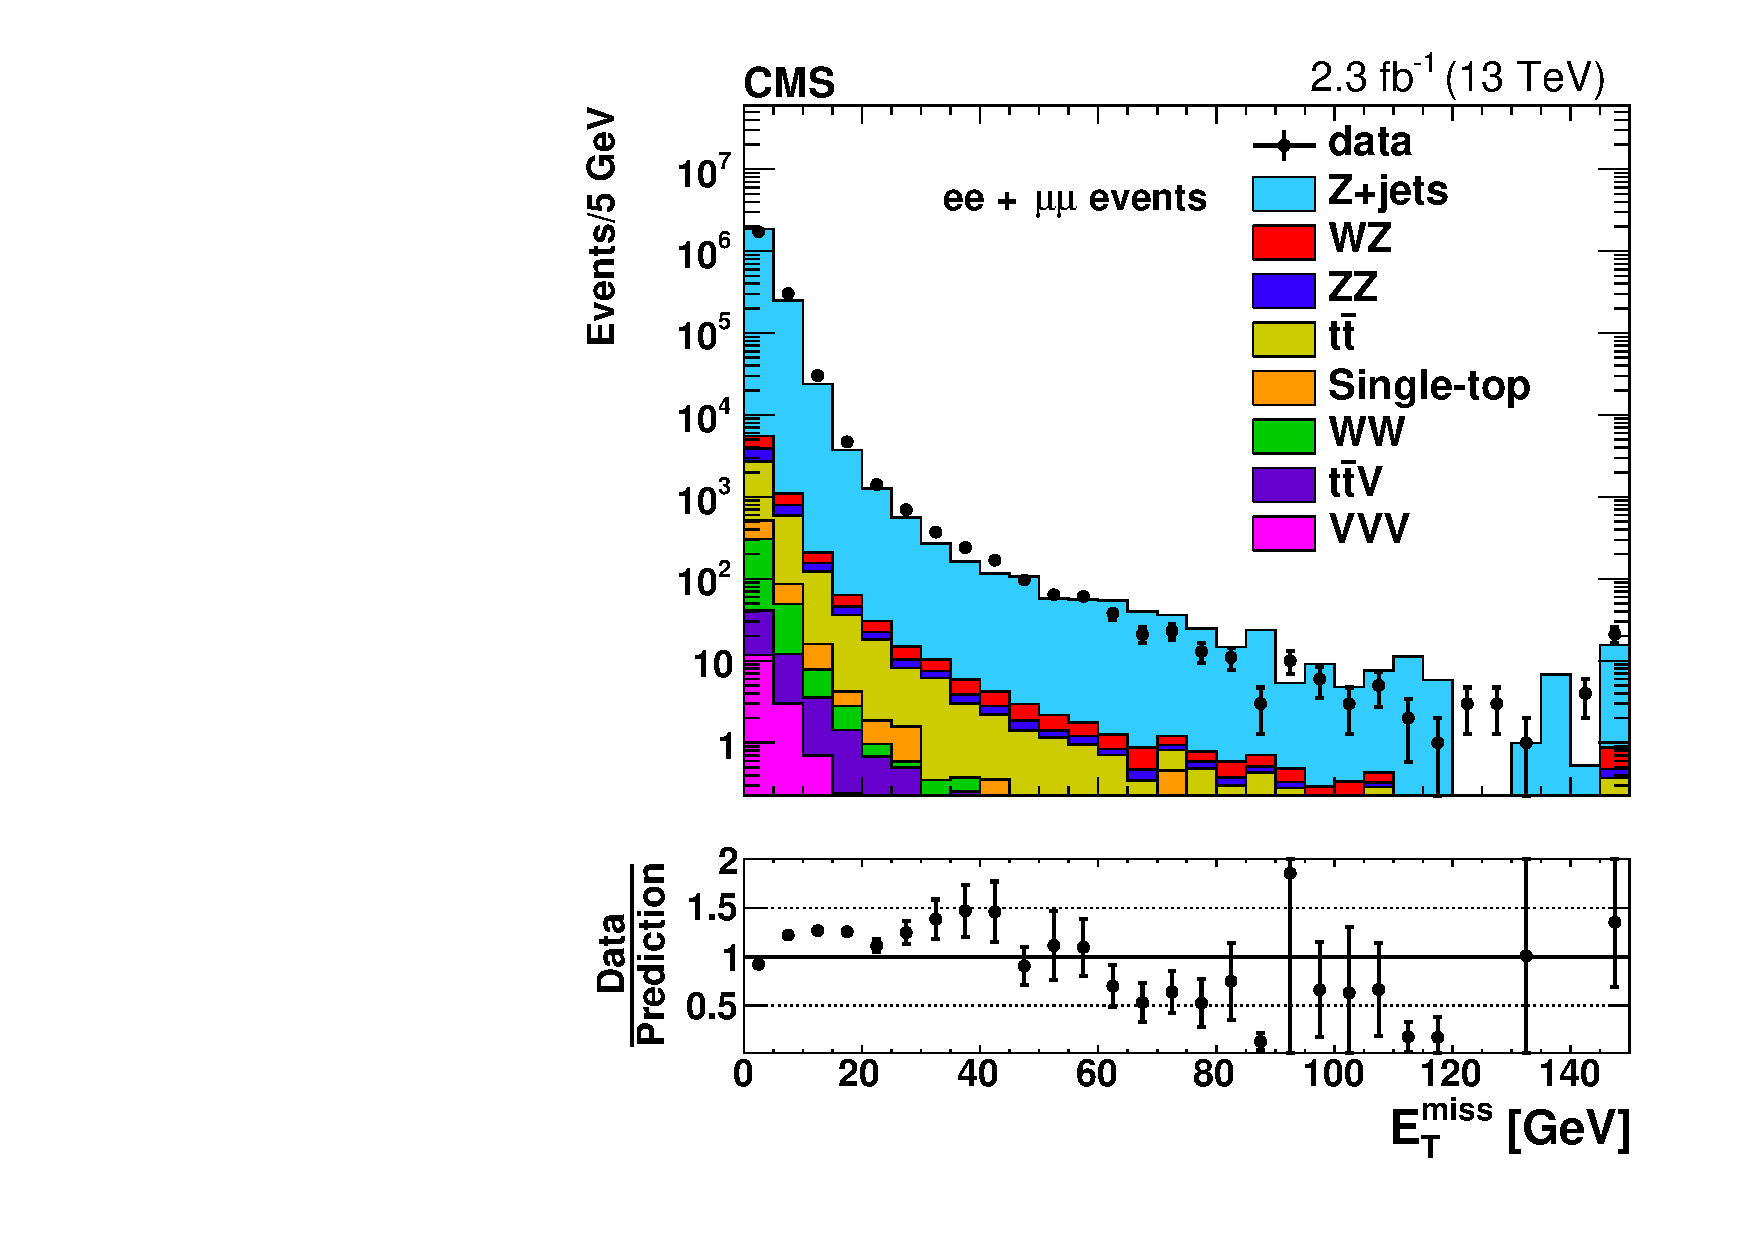
\includegraphics[width=0.4\textwidth]{MET/figs/h_met_nupfcands_1316_pt_ll_signalregion_inclusive_passtrig.pdf} \\
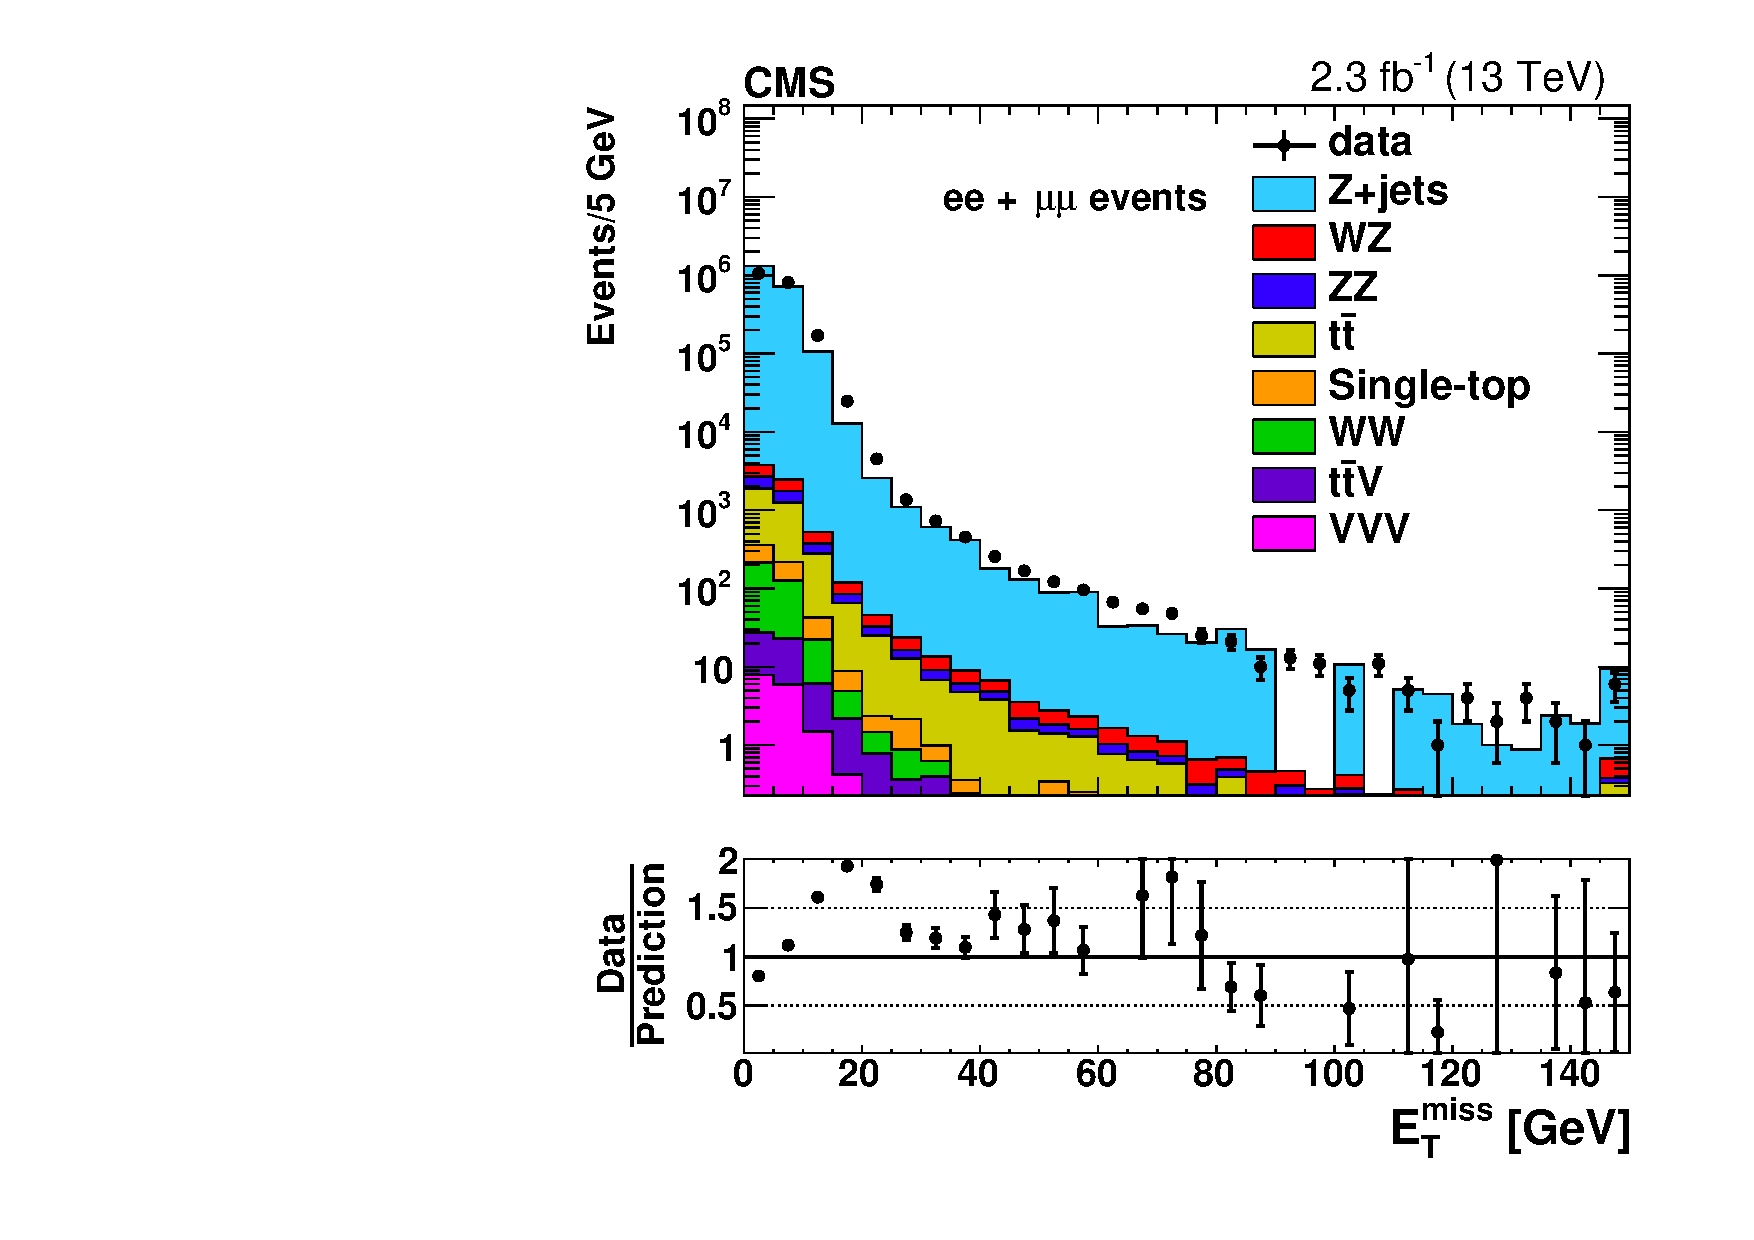
\includegraphics[width=0.4\textwidth]{MET/figs/h_met_nupfcands_1624_pt_ll_signalregion_inclusive_passtrig.pdf} &
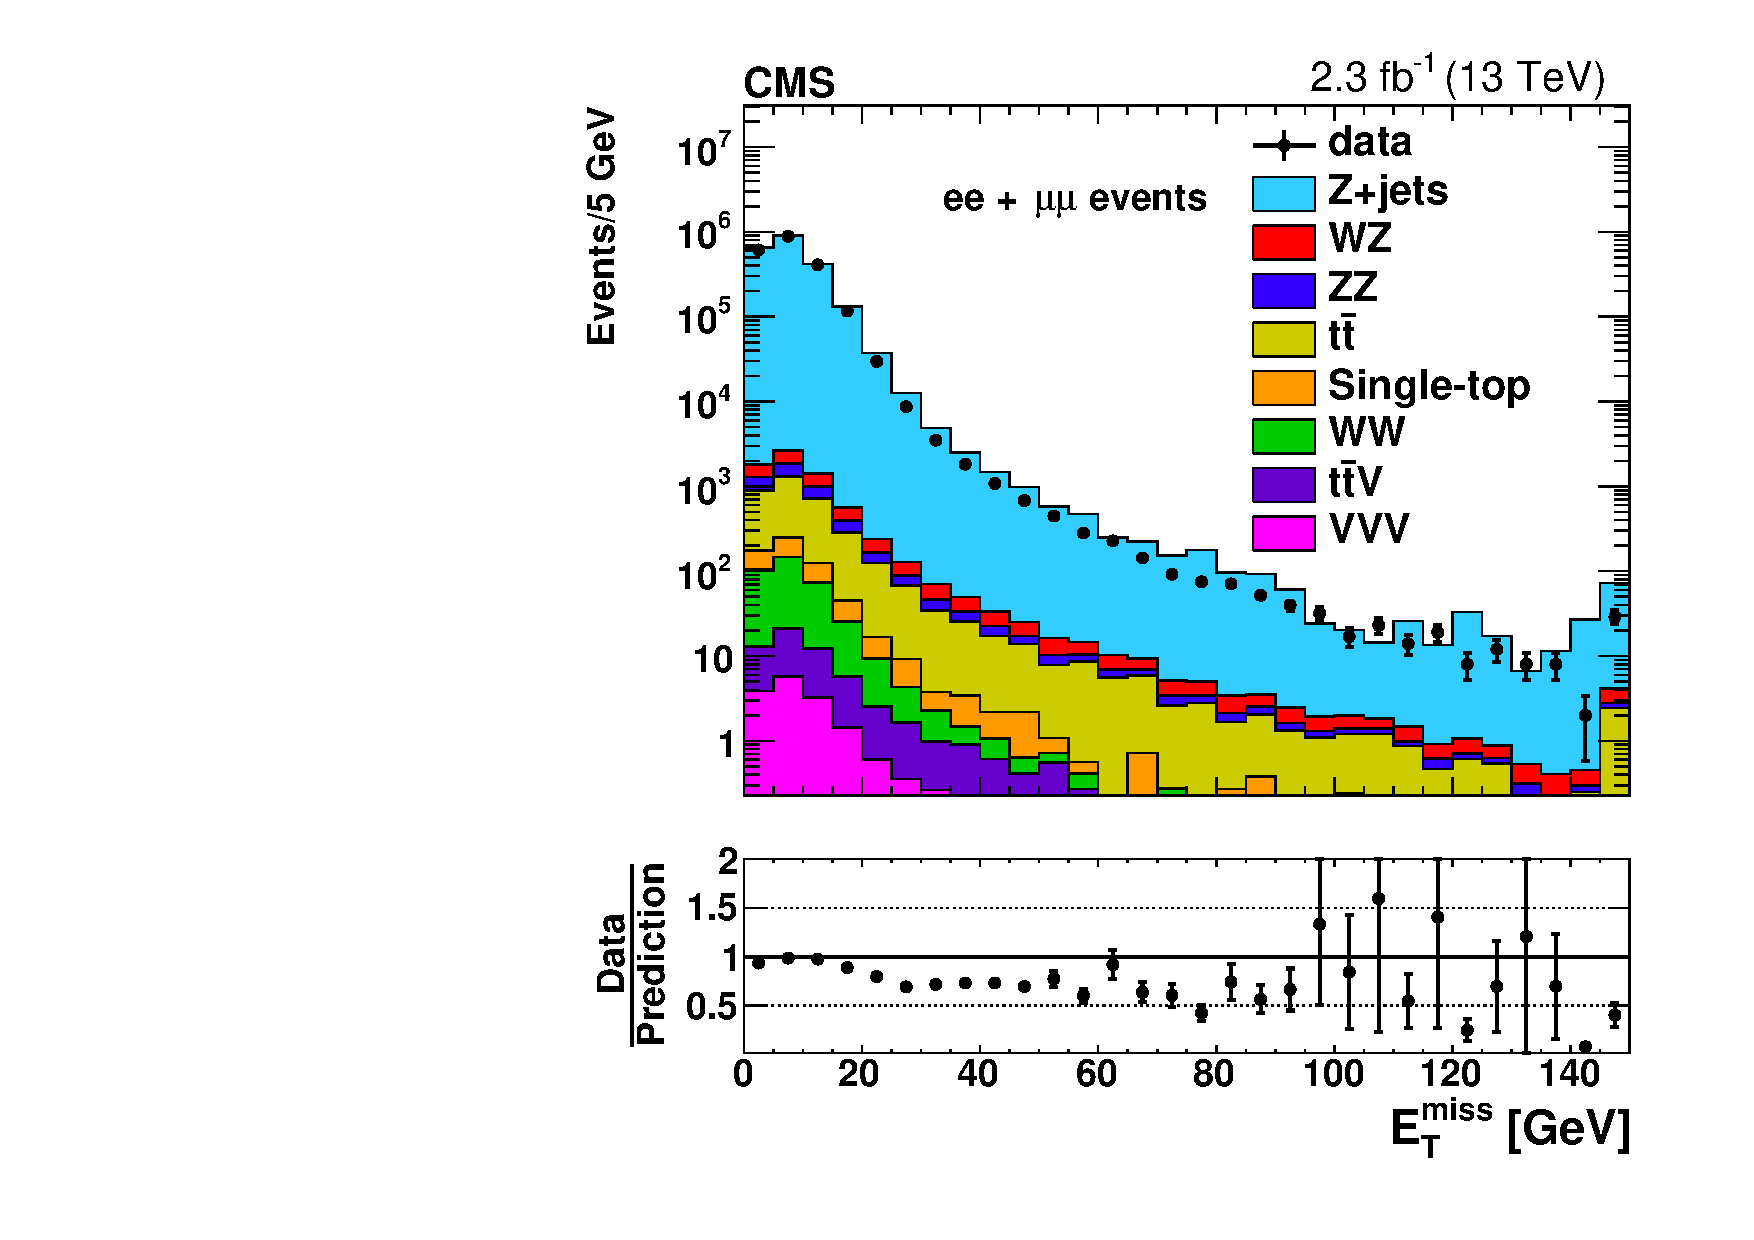
\includegraphics[width=0.4\textwidth]{MET/figs/h_met_nupfcands_2430_pt_ll_signalregion_inclusive_passtrig.pdf} \\
\end{tabular}
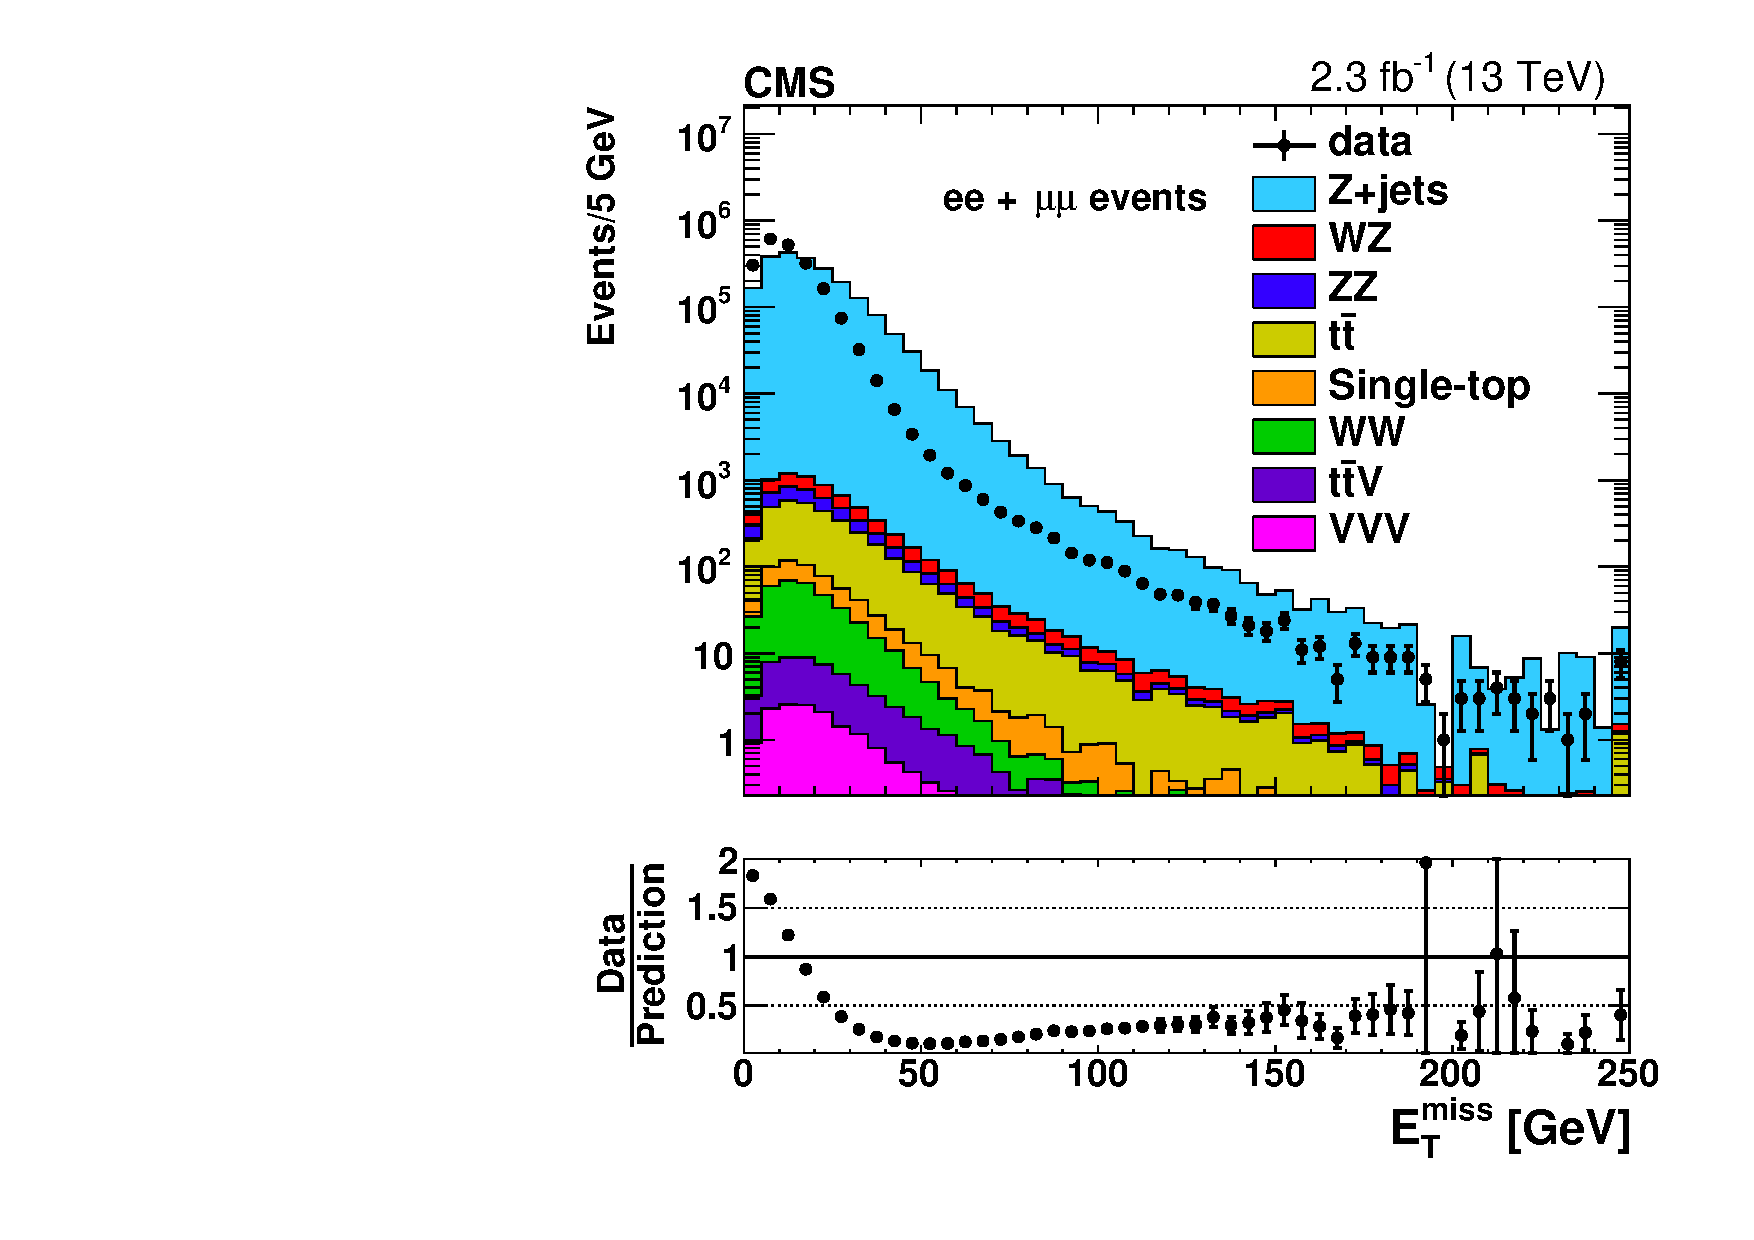
\includegraphics[width=0.4\textwidth]{MET/figs/h_met_nupfcands_30in_pt_ll_signalregion_inclusive_passtrig.pdf} 
\caption{The \MET\ distribution is shown for neutral hadronic PF candidates only.
The top row shows the barrel region on the left and transition region between the barrel and endcap on the right,
the second row shows the endcap region including the tracker on the left and endcap region excluding the tracker on the right
and the bottom row shows the HF region only.
\label{fig:nupfcands}
}
\end{center}
\end{figure}

\clearpage
